% Autor: Carles Marín (Claude, Anthropic, como asistente de investigación IA).
% Parte III. La carga del centro regresa: la muesca de m par de la torre de líneas de Wilson,
% la dicotomía de paridad, y por qué el dominio fundamental de dos Higgs no se transfiere a la
% clase admisible. Narrativa hilada por preguntas; honesta sobre el alcance. Compilar: pdflatex x2.
\documentclass[11pt,a4paper]{article}
\usepackage[utf8]{inputenc}
\usepackage[T1]{fontenc}
\usepackage[spanish,es-noshorthands]{babel}
\usepackage{amsmath,amssymb,amsthm}
\usepackage{booktabs}
\usepackage[table,dvipsnames]{xcolor}
\usepackage{graphicx}
\usepackage{tikz}
\usetikzlibrary{shapes.geometric,arrows.meta,positioning,fit,backgrounds,patterns,calc}
\usepackage{geometry}
\geometry{margin=2.4cm}
\usepackage[colorlinks=true,linkcolor=RoyalBlue,citecolor=BrickRed,urlcolor=RoyalBlue]{hyperref}
\usepackage{caption}
\captionsetup{font=small,labelfont=bf}
\newtheorem{teorema}{Teorema}
\newtheorem{lema}{Lema}
\newtheorem{corolario}{Corolario}
\newcommand{\ZZ}{\mathbb{Z}}
\newcommand{\RR}{\mathbb{R}}
\newcommand{\su}[1]{SU(#1)}
\newcommand{\lam}{|\lambda|}
\definecolor{okgreen}{RGB}{0,140,54}
\definecolor{hdrblue}{RGB}{31,78,121}
\definecolor{softgrey}{RGB}{238,242,247}
\definecolor{warmred}{RGB}{178,34,34}

\title{\textbf{\Large Una Regla de Selección por Carga del Centro\\ para el Potencial de la Línea de Wilson}\\[7pt]
\large\textnormal{\itshape El dominio fundamental de la unificación gauge--Higgs\\
depende de la representación}\\[8pt]
\normalsize\textnormal{Parte III --- selección por paridad del centro, un desacoplamiento exacto,\\
y la puerta que regalamos}}
\author{Carles Mar\'in\thanks{Investigador independiente, \texttt{karlesmarin@gmail.com}.
Los cálculos se realizaron y contrastaron con Claude (Anthropic) como asistente de
investigación IA contra una verdad-base verificable por máquina (aritmética racional exacta
sobre los sistemas de pesos de $SU(n)$ en SageMath, y un certificado en Lean~4 libre de
\texttt{sorry} para el teorema central); todo número de este trabajo se regenera desde los
scripts anexos.}}
\date{\today\\[2pt]\small DOI: \href{https://doi.org/10.5281/zenodo.21438227}{10.5281/zenodo.21438227}}

\begin{document}
\maketitle

\begin{abstract}
\noindent
La Parte~II regaló una puerta. Su primera cláusula --- que una representación puede exhibir
las hipercargas fraccionarias del Modelo Estándar solo si su carga del centro $\ZZ_4$
$a+2b+3c$ es impar --- fue identificada como la congruencia clásica de carga del centro y
declinada: \emph{no reclamamos nada de ello}. Este trabajo muestra que la puerta declinada no
es en absoluto un enunciado sobre la materia. Gobierna el sector de Higgs, y por una razón que
cabe en una línea: \emph{avanzar la línea de Wilson un periodo es, salvo una reflexión de
Weyl, multiplicar por el elemento central $-\mathbf{1}\in Z(SU(4))$ --- y la carga del centro
es, por definición, el modo en que una representación responde a uno.} Escribiendo
$D(t)=\sum_{\text{pesos}} t^{\,n_2-n_4}(-1)^{n_3}$ para la función generatriz con signo de
las etiquetas de twist del orbifold --- una proyección que aquí \emph{derivamos} de las
condiciones de contorno de $T^2/\ZZ_2$ en vez de importarla --- el carácter hereda la
respuesta del centro en la forma
$D(-t)=(-1)^{a+2b+3c}D(t)$, y con ella una dicotomía: una representación empareja sus
multiplicidades de twist de Kaluza--Klein en $m$ \emph{par} cuando la carga del centro es
impar, y en $m$ \emph{impar} cuando es par --- nunca ambas, salvo en una clase degenerada
$\mathcal Z$ que clasificamos exactamente y certificamos en Lean. El caso de $m$ impar no es
nuestro: es la hipótesis que Akamatsu, Hirose, Maru y Nago verifican inspeccionando su
Tabla~1 para reducir a la mitad el dominio fundamental de la línea de Wilson, hasta
$\alpha_2\in[0,\tfrac12]$. Como la puerta de la Parte~II fuerza la carga del centro a ser
\emph{impar} para toda representación capaz de alojar una generación de quarks, mientras que
el adjunto gauge es inevitablemente \emph{par}, la hipótesis se invierte precisamente sobre
la clase física: verificamos directamente que el potencial de toda representación admisible
viola el periodo~$1$ en $\alpha_2$ en un $2$--$30\%$ de su propia escala, de modo que la
reducción a medio dominio no se transfiere y hay que barrer el toro completo. Lo que la clase
admisible recibe a cambio es un desacoplamiento exacto: la muesca aniquila la contribución
entera de la representación fermiónica al orden dominante de Kaluza--Klein de la curvatura en
$\alpha_2=\tfrac12$, dejando una constante puramente gauge idéntica en las ocho
representaciones admisibles. El orden dominante es por tanto degenerado \emph{por teorema},
toda distinción entre representaciones candidatas vive en los términos subdominantes, y una
ordenación por naturalidad construida sobre estimaciones puntuales es frágil por una razón
estructural y no numérica. Cerramos sustituyendo el hessiano por diferencias finitas por una
medida integral de la geometría de la cuenca, validada contra él allí donde es fiable y
estable allí donde no lo es. Por último, el mecanismo no es ni un accidente ni universal: el
desplazamiento iguala a un elemento central solo cuando las posiciones neutras frente a la
línea de Wilson portan signos de twist equilibrados, lo que para una única dirección de línea
de Wilson exige $N$ par --- de modo que $SU(4)$ es el grupo más pequeño capaz de portar esta
regla de selección.
\end{abstract}

% ===================================================================
\section{La puerta que regalamos}\label{sec:intro}
Este trabajo trata sobre una frase de su predecesor.

% MOVED-FIG1: placed early so the geometry precedes the roadmap
\begin{figure}[t]
\centering
\begin{tikzpicture}[font=\small,x=1.05cm,y=1.05cm]
% ---------- (a) the flat fundamental domain ----------
\begin{scope}
\fill[softgrey] (0,0) rectangle (4,4);
\fill[RoyalBlue!13] (0,0) rectangle (2,4);
\draw[pattern=north east lines,pattern color=RoyalBlue!45,draw=none] (0,0) rectangle (2,4);
\draw[thick,black!55] (0,0) rectangle (4,4);
\draw[dashed,thick,RoyalBlue!75] (2,0) -- (2,4);
% basis vectors
\draw[-{Stealth[length=2.6mm]},very thick,BrickRed] (0,0) -- (1.15,0) node[below,pos=0.62,font=\footnotesize]{$x^5$};
\draw[-{Stealth[length=2.6mm]},very thick,okgreen!70!black] (0,0) -- (0,1.15) node[left,pos=0.62,font=\footnotesize]{$x^6$};
% edge identifications
\draw[{Stealth[length=2.2mm]}-{Stealth[length=2.2mm]},okgreen!70!black,thick] (-0.34,1.5) -- (-0.34,2.5);
\draw[{Stealth[length=2.2mm]}-{Stealth[length=2.2mm]},okgreen!70!black,thick] (4.34,1.5) -- (4.34,2.5);
\node[okgreen!55!black,font=\scriptsize,rotate=90] at (-0.62,2.0) {$U_6$};
\draw[{Stealth[length=2.2mm]}-{Stealth[length=2.2mm]},BrickRed,thick] (1.5,-0.34) -- (2.5,-0.34);
\draw[{Stealth[length=2.2mm]}-{Stealth[length=2.2mm]},BrickRed,thick] (1.5,4.34) -- (2.5,4.34);
\node[BrickRed,font=\scriptsize] at (2.0,-0.62) {$U_5=\mathbf{1}$};
% the four fixed points
\foreach \x/\y/\lb/\pv in {0/0/{P_0}/{(+,+,+,-)}, 0/2/{P_2}/{(+,+,-,-)},
                            2/0/{P_1}/{(+,+,+,-)}, 2/2/{P_3}/{(+,+,-,-)}}{
  \fill[hdrblue] (\x,\y) circle (2.6pt);
  \node[hdrblue,font=\scriptsize,above right=0pt and 1pt] at (\x,\y) {$\lb$};
}
\node[font=\scriptsize,black!65,align=center] at (2.0,4.95)
  {$P_0=P_1=\mathrm{diag}(+,+,+,-)$\\[-1pt]$P_2=P_3=\mathrm{diag}(+,+,-,-)$};
\node[RoyalBlue!85,font=\scriptsize,align=center] at (1.0,-1.15) {dominio fundamental\\[-1pt]de $\ZZ_2$};
\node[font=\small\bfseries] at (2.0,-1.85) {(a)};
\end{scope}
% ---------- (b) the pillow ----------
\begin{scope}[shift={(6.6,0.35)}]
\fill[softgrey,rounded corners=20pt] (0,0.3) .. controls (0.4,3.6) and (3.0,3.9) .. (3.4,1.6)
   .. controls (3.6,0.4) and (1.2,-0.5) .. (0,0.3) -- cycle;
\draw[thick,black!55] (0,0.3) .. controls (0.4,3.6) and (3.0,3.9) .. (3.4,1.6)
   .. controls (3.6,0.4) and (1.2,-0.5) .. (0,0.3) -- cycle;
\draw[black!25,thin] (0.15,1.4) .. controls (1.2,2.2) and (2.4,2.1) .. (3.35,1.5);
\draw[black!25,thin] (1.15,0.0) .. controls (1.5,1.2) and (1.5,2.4) .. (1.2,3.35);
\foreach \x/\y/\lb in {0.02/0.32/{P_0}, 1.62/3.55/{P_2}, 3.42/1.6/{P_1}, 1.10/-0.32/{P_3}}{
  \fill[hdrblue] (\x,\y) circle (2.6pt);
  \node[hdrblue,font=\scriptsize,inner sep=2pt] at (\x+0.36,\y+0.20) {$\lb$};
}
\node[font=\scriptsize,black!65,align=center] at (1.7,-1.5) {el cociente: una almohada con\\[-1pt]cuatro puntos fijos cónicos};
\node[font=\small\bfseries] at (1.7,-2.2) {(b)};
\end{scope}
\end{tikzpicture}
\caption{\textbf{La geometría sobre la que vive toda figura posterior.} \textbf{(a)} El toro
$T^2$ con el dominio fundamental de $\ZZ_2$ rayado. Las traslaciones alrededor de los dos
ciclos van acompañadas de $U_5$ y $U_6$; invertir las relaciones de consistencia de AHMN
$P_1=U_5P_0$, $P_2=U_6P_0$ da $U_5=\mathbf{1}$ y $U_6=\mathrm{diag}(1,1,-1,1)$, que es el
origen entero de la etiqueta de twist $q$ (\S\ref{sec:projection}). Los cuatro puntos fijos de
$\ZZ_2$ portan las matrices de paridad mostradas; nótese $P_0=P_1$ y $P_2=P_3$, de modo que
solo la dirección $x^6$ porta un twist discreto --- la asimetría visible
en~\eqref{eq:twists}. \textbf{(b)} El cociente $T^2/\ZZ_2$: una almohada con cuatro puntos
cónicos, uno por punto fijo. Todo mapa de calor de este trabajo es la imagen plana de (a),
dibujada sobre el rango completo de periodo~$2$ de las fases de la línea de Wilson.}
\label{fig:fundamental}
\end{figure}

La Parte~I~\cite{PartI} retomó una pregunta abierta desde 2003 --- Scrucca, Serone,
Silvestrini y Wulzer habían observado que en un orbifold la cancelación de anomalías y la
anulación de los tadpoles localizados son requisitos \emph{independientes}, y nombraron la
pieza que faltaba como un problema abierto~\cite{SSSW} --- y la abordó dentro del modelo
$SU(4)$ six-dimensional de dos dobletes de Higgs de Akamatsu, Hirose, Maru y
Nago~\cite{AHMN}: un bloque coloreado de quarks en la representación de dimensión $60$, una
completación de $45$ multipletes que cancela anomalías y tadpole juntos, y un teorema de
Existencia que muestra que el tadpole nunca obstruye. La Parte~II~\cite{PartII} convirtió la
minimalidad que la Parte~I meramente había observado en una ley exacta: una irreducible
$(a,b,c)$ de $SU(4)$ contiene una celda de quarks del Modelo Estándar entre sus modos cero
quirales de $T^2/\ZZ_2$ si y solo si
\begin{equation}\label{eq:criterion}
(a+2b+3c)\ \text{impar}\quad\wedge\quad b\ge1\quad\wedge\quad a+b+c\ge3 .
\end{equation}
La Parte~II fue cuidadosa con el crédito, y en ningún sitio más que en la primera cláusula.
La carga del centro $\ZZ_4$ --- la clase de congruencia de Slansky $c(R)=a+2b+3c \bmod
4$~\cite{Slansky} --- ata la hipercarga fraccionaria a una congruencia fija, un hecho
enunciado para el propio $\ZZ_6$ del Modelo Estándar por Hucks y por Saller y reformulado en
lenguaje de estructura global por Tong y por Alonso, Dimakou y
West~\cite{Hucks,Saller,Tong,Alonso}. La Parte~II escribió, con todas las letras, \emph{``no
reclamamos nada de ello''}, y registró la cláusula como \emph{heredada, no inventada}.

Regalarla fue lo correcto, y la razón es larga. La observación de que el \emph{centro} de un
grupo gauge porta física que el álgebra por sí sola no porta se remonta a la condición de
cuantización de Dirac y fue afilada por la clasificación de fases de 't~Hooft según las
cargas eléctricas y magnéticas que la sobreviven~\cite{tHooft}: qué admite una teoría como
operador de línea, y qué cargas fraccionarias puede portar, no lo decide $\mathfrak{su}(n)$
sino qué cociente del grupo simplemente conexo se gauge\'a. Hucks y Saller sacaron la
conclusión correspondiente para el propio Modelo Estándar --- su verdadero grupo gauge es
$\big(SU(3)\times SU(2)\times U(1)\big)/\ZZ_6$, y las hipercargas familiares
$\tfrac16,\tfrac23,-\tfrac13$ son precisamente las fracciones que ese cociente
permite~\cite{Hucks,Saller}. Tong reformuló el enunciado en el lenguaje de los operadores de
línea~\cite{Tong}, y Alonso, Dimakou y West plantearon la pregunta experimental escondida
dentro de él --- qué estados de carga fraccionaria distinguirían entre los grupos
candidatos~\cite{Alonso}. Para cuando la Parte~II necesitó el hecho, este había sido
establecido cuatro veces distintas en cuatro lenguajes distintos. Una cosa así no se reclama.

Aquello era correcto, y este trabajo no se retracta. Pero era incompleto de un modo que no
sospechábamos, porque dejó una pregunta sin hacer. La carga del centro entró
en~\eqref{eq:criterion} como una condición \emph{aritmética} sobre el sector de materia: qué
pesos pueden portar $\tfrac16,\tfrac23,-\tfrac13$ siquiera. Nada en esa derivación sugiere
que la misma congruencia deba tener algo que decir sobre el sector de \emph{Higgs} --- sobre
el potencial de la línea de Wilson, sus simetrías, su vacío, o la masa que genera. Ambos
viven en partes distintas de la construcción y se calculan a partir de datos distintos.

Así pues: \emph{¿sabe la carga del centro algo del potencial de Higgs?} La respuesta es que
lo controla, en un sentido que podemos hacer exacto. No reclamamos la congruencia. Reclamamos
lo que hace --- y lo que hace no es una restricción sobre la materia sino una restricción
sobre el \emph{potencial mismo}.

\begin{center}
\fcolorbox{hdrblue}{RoyalBlue!6}{\parbox{0.94\textwidth}{%
\vspace{3pt}
\textbf{Principio de Selección por Paridad del Centro.}\ \ Sea un desplazamiento de un módulo
de línea de Wilson equivalente, salvo Weyl, a la multiplicación por un elemento central
$\zeta$ de orden $d$. Entonces el soporte de Fourier del potencial a un loop se escinde en
$d$ sectores etiquetados por la carga del centro módulo $d$, y una representación $R$
contribuye a un sector solo allí donde $\zeta^{\,c(R)}=1$. Los sectores en que
$\zeta^{\,c(R)}\neq1$ son \emph{idénticamente vacíos} para esa representación --- no
suprimidos: ausentes.
\smallskip

\textbf{El caso aquí demostrado} es $SU(4)$ sobre $T^2/\ZZ_2$, donde $\zeta=-\mathbf{1}$
tiene $d=2$ y la carga es $c(R)=a+2b+3c$: un bit, leído en cuatro sitios ---
\emph{admisibilidad de la materia}, \emph{emparejamiento de twists de Kaluza--Klein}, el
\emph{soporte de Fourier} del potencial y la \emph{geometría de su vacío}.
\vspace{3pt}}}
\end{center}

\noindent
La carga del centro se ha usado durante medio siglo como condición sobre qué
\emph{representaciones} pueden portar hipercarga fraccionaria; aquí decide además qué
\emph{armónicos} del potencial de Hosotani pueden siquiera existir. La
Figura~\ref{fig:chain} dibuja el centro del grupo en el centro de la página, con los cuatro
sectores que gobierna a su alrededor.

\begin{figure}[!t]
\centering
\begin{tikzpicture}[font=\small,
  pan/.style={rounded corners=3pt,draw,thick,align=center,inner sep=6pt,
              text width=3.45cm,fill=white,draw=black!35},
  ttl/.style={font=\footnotesize\bfseries},
  ray/.style={-{Stealth[length=2.6mm]},thick,black!45}]

% ---------------- the centre of the group, at the centre of the figure ----------------
\begin{scope}
\fill[RoyalBlue!6] (0,0) circle (2.22);
\draw[RoyalBlue!50,thick] (0,0) circle (1.90);
\foreach \a/\lb in {90/{1}, 0/{i}, 270/{-i}}
  {\fill[black!55] (\a:1.90) circle (2.2pt);
   \node[font=\scriptsize,black!55] at (\a:2.18) {$\lb$};}
\fill[BrickRed] (180:1.90) circle (3.6pt);
\node[font=\scriptsize\bfseries,BrickRed] at (180:2.30) {$-\mathbf{1}$};
% the half turn: one period of Wilson line
\draw[-{Stealth[length=2.6mm]},very thick,BrickRed] (84:1.90) arc (84:174:1.90);
\node[font=\scriptsize,BrickRed,align=center] at (0,2.70) {un periodo de $\alpha_2$};
% the answer, on a clean backing so nothing collides
\node[fill=white,rounded corners=2pt,inner sep=4pt,align=center,font=\scriptsize] at (0,0)
  {el centro\\[1pt]
   $Z\cong\ZZ_4$\\[4pt]
   responde con\\[1pt]
   $(-1)^{a+2b+3c}$\\[4pt]
   {\itshape un bit}};
\end{scope}

% ---------------- the four faces ----------------
% (1) matter
\node[pan] (p1) at (-5.0, 2.35)
  {\footnotesize\bfseries\ materia\\[3pt]
   \begin{tikzpicture}[scale=0.42,baseline]
     \draw[black!30] (-0.2,0)--(3.4,0);
     \foreach \x/\y/\lb in {0.35/1.10/{\tfrac23}, 1.75/0.28/{\tfrac16}, 3.15/-0.55/{-\tfrac13}}
       {\fill[RoyalBlue!75] (\x,\y) circle (5pt);
        \node[font=\tiny,above=1pt] at (\x,\y) {$\lb$};}
   \end{tikzpicture}\\[2pt]
   {\scriptsize qué reps.\ portan las fracciones del ME}\\[1pt]
   {\scriptsize\itshape Parte~II \textperiodcentered\ clásico}};
% (2) twist pairing
\node[pan] (p2) at (-5.0,-2.35)
  {\footnotesize\bfseries\ emparejamiento\\ de twists\\[3pt]
   \begin{tikzpicture}[scale=0.42,baseline]
     \draw[black!30] (-0.1,0)--(3.5,0);
     \foreach \x in {0.3,1.1,1.9,2.7} \draw[okgreen!75!black,line width=2.2pt] (\x,0)--(\x,0.95);
     \foreach \x in {0.7,1.5,2.3,3.1} \draw[black!22,line width=2.2pt,dashed] (\x,0)--(\x,0.55);
   \end{tikzpicture}\\[2pt]
   {\scriptsize qué peine de $(m,q)$ equilibra}\\[1pt]
   {\scriptsize\itshape \S\ref{sec:dichotomy}}};
% (3) Fourier support
\node[pan] (p3) at (5.0, 2.35)
  {\footnotesize\bfseries\ soporte de Fourier\\[3pt]
   \begin{tikzpicture}[scale=0.42,baseline]
     \foreach \x in {0,...,4} \foreach \y in {0,...,3}
       {\pgfmathparse{int(mod(\y,2))}\ifnum\pgfmathresult=0
          \fill[RoyalBlue!70] (\x*0.8,\y*0.42) circle (3.6pt);
        \else
          \draw[black!25] (\x*0.8,\y*0.42) circle (3.6pt);
        \fi}
   \end{tikzpicture}\\[2pt]
   {\scriptsize qué armónicos de $V$ pueden existir}\\[1pt]
   {\scriptsize\itshape \S\ref{sec:dichotomy} \textperiodcentered\ Fig.~\ref{fig:spectrum}}};
% (4) vacuum geometry
\node[pan] (p4) at (5.0,-2.35)
  {\footnotesize\bfseries\ geometría del vacío\\[3pt]
   \begin{tikzpicture}[scale=0.42,baseline]
     \fill[softgrey] (0,0) rectangle (3.2,1.6);
     \draw[black!45] (0,0) rectangle (3.2,1.6);
     \draw[BrickRed,thick,dashed] (0,0.8)--(3.2,0.8);
     \node[font=\tiny,BrickRed] at (1.6,0.42) {medio};
     \node[font=\tiny,black!60] at (1.6,1.2) {todo};
   \end{tikzpicture}\\[2pt]
   {\scriptsize qué dominio hay que barrer}\\[1pt]
   {\scriptsize\itshape \S\S\ref{sec:domain},\,\ref{sec:decoupling}}};

\foreach \p in {p1,p2,p3,p4} \draw[ray] (0,0) -- (\p);
\end{tikzpicture}
\caption{\textbf{El centro del grupo, en el centro de la imagen.} Un periodo de la línea de
Wilson es media vuelta del centro $\ZZ_4$ --- aterriza en $-\mathbf{1}$ --- y una
representación responde a ese elemento con el único bit $(-1)^{a+2b+3c}$. Todo lo que este
trabajo demuestra es ese bit leído en cuatro sitios: qué representaciones pueden portar las
hipercargas del Modelo Estándar (conocido, y declinado en la Parte~II), qué peine de
multiplicidades de twist equilibra, qué armónicos del potencial de la línea de Wilson tienen
permitido ser no nulos siquiera, y cuánto toro hay que barrer en busca de su vacío. Parecen
cuatro hechos distintos sobre un modelo. Son un hecho sobre un grupo.}
\label{fig:chain}
\end{figure}

\paragraph{Alcance y relación con trabajo previo.} Como en la Parte~II separamos lo heredado
de lo nuevo, y de nuevo la mayoría de los ingredientes son heredados. La congruencia de carga
del centro es clásica~\cite{Hucks,Saller,Tong,Alonso,Slansky}. La construcción del orbifold,
las etiquetas de twist $(m,q)$, la ecuación de masa, el potencial a un loop y el argumento del
dominio fundamental son todos de AHMN~\cite{AHMN}; citamos su Sección~4.3 literalmente en
\S\ref{sec:domain} porque nuestra afirmación física central es sobre el alcance de \emph{su}
hipótesis, no sobre un error en ella --- su argumento es correcto para su modelo. El
mecanismo tras nuestro teorema de anulación es asimismo clásico: el alfabeto
$\{1,-1,t,t^{-1}\}$ tiene determinante $-1$, de modo que parametriza la componente impropia
de $O(4)$, donde una representación irreducible y su asociada $\mu\otimes\det$ tienen
caracteres opuestos y las autoasociadas se anulan~\cite{Brauer}; la ramificación es la regla
de restricción de Littlewood con las reglas de modificación de Newell--King~\cite{King71,Newell,Brauer},
y la técnica del determinante que usamos la describen Ayyer y Behrend como
rutinaria~\cite{AyyerBehrend}. Lo nuestro es cuádruple: (i) la \emph{dicotomía}
(\S\ref{sec:dichotomy}) y la clasificación exacta de su clase degenerada
(\S\ref{sec:degenerate}), certificada por máquina en Lean~4; (ii) la observación --- con
verificación directa --- de que la reducción de dominio fundamental de AHMN \emph{se
invierte} sobre la clase admisible para el Modelo Estándar (\S\ref{sec:domain}); (iii) el
corolario de \emph{desacoplamiento} y la degeneración de orden dominante resultante
(\S\ref{sec:decoupling}); y (iv) una derivación de la proyección $(m,q)$ a partir de las
condiciones de contorno (\S\ref{sec:projection}), que en esta construcción se venía usando
como un input calibrado. La Figura~\ref{fig:roadmap} es la ruta.

\emph{Establecido aquí:} el principio --- un período de línea de Wilson es una transformación
gauge central, de modo que la carga del centro es un enunciado sobre el potencial y no solo
sobre la materia. \emph{Abierto:} sus cuatro lecturas, que son el resto del trabajo.



\begin{figure}[t]
\centering
\resizebox{0.82\textwidth}{!}{%
\begin{tikzpicture}[font=\small,
  act/.style={rounded corners,draw,thick,text width=3.5cm,align=center,inner sep=6pt,minimum height=4.3cm,anchor=north},
  arr/.style={-{Stealth[length=3.4mm]},very thick,black!55}]
\node[act,fill=RoyalBlue!8,draw=RoyalBlue!65] (a1) at (0,0)
 {\textbf{I.\ Una}\\[1pt]{\footnotesize Parte I}\\[5pt]
  \textit{un testigo: anomalías}\\\textit{y tadpole cancelan}\\\textit{juntos}\\[6pt]
  {\footnotesize\color{RoyalBlue}\textbf{existencia}}};
\node[act,fill=okgreen!9,draw=okgreen!65] (a2) at (5.6,0)
 {\textbf{II.\ Todas}\\[1pt]{\footnotesize Parte II}\\[5pt]
  \textit{qué $(a,b,c)$ alojan}\\\textit{una generación de quarks}\\[6pt]
  {\footnotesize$(a{+}2b{+}3c)$ impar\\$\wedge\,b\ge1\wedge a{+}b{+}c\ge3$}\\[4pt]
  {\footnotesize\color{okgreen}\textbf{puerta 1: ``no reclamamos nada''}}};
\node[act,fill=warmred!8,draw=warmred!70] (a3) at (11.2,0)
 {\textbf{III.\ La puerta vuelve}\\[1pt]{\footnotesize este trabajo}\\[5pt]
  \textit{la misma paridad rige}\\\textit{la torre de la línea de Wilson}\\[6pt]
  {\footnotesize $D(-t)=(-1)^{\lam}D(t)$}\\[4pt]
  {\footnotesize\color{warmred}\textbf{una dicotomía}}};
\node[act,fill=softgrey,draw=hdrblue!65] (a4) at (16.8,0)
 {\textbf{IV.\ El precio}\\[1pt]{\footnotesize \S\S\,5--6}\\[5pt]
  \textit{el medio dominio de}\\\textit{AHMN se invierte; el orden}\\\textit{dominante desacopla}\\[6pt]
  {\footnotesize\color{hdrblue}\textbf{barrer el toro completo}}};
\draw[arr] (a1.east) -- node[above,font=\footnotesize\itshape,black!70]{generaliza} (a2.west);
\draw[arr] (a2.east) -- node[above,font=\footnotesize\itshape,black!70]{re-pregunta} (a3.west);
\draw[arr] (a3.east) -- node[above,font=\footnotesize\itshape,black!70]{paga} (a4.west);
\end{tikzpicture}}
\caption{El arco de la serie. La Parte~I produjo un único modelo consistente; la Parte~II la
ley exacta de qué representaciones son elegibles, declinando explícitamente su puerta
aritmética como clásica. Este trabajo pregunta qué hace esa puerta declinada en otro lugar, y
la encuentra gobernando el potencial gauge--Higgs --- con una consecuencia que hay que pagar
antes de calcular vacío alguno en esta clase.}
\label{fig:roadmap}
\end{figure}

% ===================================================================
\section{De dónde vienen las etiquetas de twist}\label{sec:projection}
Antes de poder demostrar nada sobre la torre, hay que saber exactamente qué la etiqueta.

Las etiquetas son viejas. En 1979 Scherk y Schwarz notaron que un campo sobre un espacio
compacto no tiene por qué volver a sí mismo: puede volver actuado por una simetría, y el
twist resultante da masas que ningún potencial puso ahí~\cite{ScherkSchwarz}. Ese mismo año
Manton y Fairlie observaron que las componentes extra-dimensionales de un campo gauge son
escalares en cuatro dimensiones, con un acoplo cuártico fijado por el acoplo gauge en vez de
libre~\cite{Manton,Fairlie}; Hosotani mostró después que el vacío de tal escalar es una línea
de Wilson, de modo que la ruptura de simetría pasa a ser un enunciado sobre la holonomía
alrededor de un ciclo~\cite{Hosotani}. Esa es la idea entera de la unificación gauge--Higgs:
el Higgs es un twist. Los orbifolds entraron cuando Kawamura usó una proyección $\ZZ_2$ para
partir un multiplete gran-unificado~\cite{KawamuraGUT}, y las construcciones modernas --- la
de AHMN incluida --- combinan ambas cosas, de modo que un modo porta \emph{a la vez} una fase
de línea de Wilson y una paridad discreta. Ese par de datos es exactamente lo que registra
$(m,q)$.

Por eso hay que fijar el par antes que nada. AHMN asignan a cada modo de Kaluza--Klein un par
de enteros $(m,q)$ mediante condiciones de contorno
retorcidas~\cite[Ecs.~(3.3)--(3.4)]{AHMN},
\begin{equation}\label{eq:twists}
f(x^5+2\pi R,x^6)=e^{i\pi m\alpha_1}f(x^5,x^6),\qquad
f(x^5,x^6+2\pi R)=e^{i\pi(m\alpha_2+q)}f(x^5,x^6),
\end{equation}
con $\alpha_{1,2}=gRv_{1,2}$ las fases de la línea de Wilson, $m$ ``el peso del generador'' y
$q\in\{0,1\}$ periódico o antiperiódico. En términos de las coordenadas de partición
$n=(n_1,n_2,n_3,n_4)$ de un peso, esta construcción se usa con $m=n_2-n_4$ y
$q=n_3\bmod2$. Esa asignación suele justificarse contrastándola con la Tabla~1 de AHMN.
Contrastar no es derivar, así que la derivamos.

Los datos de contorno son los de AHMN: traslaciones $U_{5,6}$, paridades $P_i$ en los cuatro
puntos fijos, y las relaciones de consistencia $P_1=U_5P_0$, $P_2=U_6P_0$~\cite[Ec.~(2.8)]{AHMN},
con la elección~\cite[Ecs.~(2.9)--(2.10)]{AHMN}
\[
P_0=P_1=\mathrm{diag}(+,+,+,-),\qquad P_2=P_3=\mathrm{diag}(+,+,-,-),
\]
que rompe $SU(4)\to SU(2)_L\times U(1)_Y\times U(1)_X$. Invirtiendo las relaciones,
\begin{equation}\label{eq:U}
U_5=P_1P_0^{-1}=\mathbf{1},\qquad
\boxed{\,U_6=P_2P_0^{-1}=\mathrm{diag}(1,1,-1,1)\,}
\end{equation}
Un estado de contenido $n$ en cualquier representación tensorial recoge por tanto
$\prod_i (U_6)_{ii}^{\,n_i}=(-1)^{n_3}$ bajo la traslación en $x^6$, que es exactamente la
alternativa periódico/antiperiódico de~\eqref{eq:twists}: $q=n_3\bmod2$. Dos comprobaciones
independientes salen gratis. Primera, $q$ no es un dato extra sino el \emph{producto de las
dos paridades $\ZZ_2$}: sobre contenido $n$, $P_0\mapsto(-1)^{n_4}$ y
$P_2\mapsto(-1)^{n_3+n_4}$, cuyo producto es $(-1)^{n_3}$, consistente con $U_6=P_2P_0$.
Segunda, y más reveladora, \eqref{eq:twists} es \emph{asimétrica} --- la condición en $x^5$
no porta $q$ y la de $x^6$ sí. AHMN no comentan esto. Es precisamente $U_5=\mathbf{1}$ frente
a $U_6\neq\mathbf{1}$: no hay twist discreto a lo largo de $x^5$ que una $q$ pueda describir.

Para $m$: las componentes de $A_{5,6}$ con modos no masivos cuadridimensionales --- las
entradas $(++)$ de~\cite[Ec.~(2.12)]{AHMN} --- se sitúan en las posiciones de matriz
$(1,4),(2,4),(4,1),(4,2)$, que son los dos dobletes de Higgs. Los valores esperados de vacío
de la línea de Wilson yacen ahí, y usar $SU(2)_L$ (actuando sobre los índices $1,2$) para
alinearse con la segunda componente del doblete hace del generador $E_{24}+E_{42}$, conjugado
dentro del bloque $\{2,4\}$ a
\begin{equation}
T=\mathrm{diag}(0,1,0,-1),
\end{equation}
cuyo peso sobre contenido $n$ es $n_2-n_4$. Que una \emph{única} $m$ aparezca en ambas
mitades de~\eqref{eq:twists} es consistente: ambos ciclos portan la misma dirección del
álgebra de Lie con magnitudes distintas $v_1,v_2$. La elección del par de índices es libertad
gauge de $SU(2)_L$, y es demostrablemente irrelevante --- la función generatriz $D$ de
\S\ref{sec:dichotomy} es invariante bajo las $24$ asignaciones $m=n_i-n_j$, $q=n_k\bmod2$ con
$i,j,k$ distintos. La libertad de la derivación y la libertad del teorema son la misma
libertad.

\paragraph{Leer la Tabla~1 correctamente.} Aplicar $(T,U_6)$ al $\mathbf{35}=(4,0,0)$ da,
para $m\ge1$, los recuentos $3,3,3,1,1,1,1$ en $(1,0),(1,1),(2,0),(2,1),(3,0),(3,1),(4,0)$,
coincidiendo con la Tabla~1 de AHMN entrada por entrada --- pero como recuentos de
\emph{multipletes} de $SU(2)_L$, no de estados. La razón es física. $T$ no conmuta con
$SU(2)_L$: mover una caja entre los índices $1$ y $2$ desplaza $n_2$, y por tanto $m$, en
uno. Un multiplete de tamaño $s$ no porta entonces una única $m$; se reparte sobre $s$
valores \emph{consecutivos}, contribuyendo exactamente un estado a cada uno. Lo verificamos
sobre el $\mathbf{35}$ sin excepciones, y la identidad ``\#pesos en $(m,q)$ $=$ \#multipletes
que abarcan $(m,q)$'' se cumple exactamente. Que la línea de Wilson parta los multipletes de
$SU(2)_L$ no es contabilidad --- es ruptura de simetría electrodébil, que es para lo que está
la línea de Wilson.

\emph{Establecido aquí:} $q$ es el twist $U_6=P_2P_0^{-1}$, equivalentemente el producto de
las dos paridades del orbifold, y $m$ es el peso bajo el generador de la línea de Wilson; la
Tabla~1 queda reproducida \emph{y} explicada. \emph{Abierto:} nada a este nivel --- lo que
sigue siendo un input es la propia elección de paridades de AHMN, que es su definición de
modelo, como debe ser.

% ===================================================================
\section{Selección por paridad del centro, y la dicotomía que fuerza}\label{sec:dichotomy}
Con las etiquetas fijadas podemos hacerle a la torre una pregunta afilada --- y el modo de
hacerla es también prestado.

Hay una vieja costumbre en teoría de representaciones: aprender sobre un carácter evaluándolo
en un elemento del grupo \emph{distinguido} en vez de estudiarlo en general. Los
\emph{Classical Groups} de Weyl están construidos sobre la técnica~\cite{Weyl}, y Littlewood
la convirtió en una máquina: dale a una función de Schur un alfabeto con estructura ---
variables en pares $\pm$, por ejemplo --- y la respuesta no es meramente más simple sino
combinatoria, anulándose sin más a menos que la partición pase un test de
divisibilidad~\cite{LittlewoodBook}. La costumbre sigue muy viva: Ciucu y Krattenthaler
hallaron que los caracteres en pares recíprocos $x,x^{-1}$
factorizan~\cite{CiucuKrattenthaler}, Ayyer y Behrend ampliaron la
clase~\cite{AyyerBehrend}, y Ayyer y Kumari clasificaron exactamente qué particiones
sobreviven a un twist por una raíz de la unidad~\cite{AyyerKumari,Kumari}. En todos los casos
el elemento especial convierte una pregunta sobre representaciones en aritmética sobre un
diagrama de Young.

Nuestra torre nos entrega tal elemento gratis. Las dos paridades del orbifold y la línea de
Wilson evalúan juntas el carácter de $SU(4)$ en un alfabeto que es mitad $\pm1$ y mitad
recíproco --- y, como veremos, ese alfabeto no es una elección cómoda sino la que dicta la
física. Así que seguimos la costumbre. Define la función generatriz con signo de las etiquetas
de twist,
\begin{equation}\label{eq:D}
D(t)\;=\;\sum_{\text{pesos}} t^{\,n_2-n_4}\,(-1)^{n_3}\;=\;s_\lambda\!\left(1,-1,t,t^{-1}\right),
\qquad \lambda=(a{+}b{+}c,\;b{+}c,\;c,\;0),
\end{equation}
la segunda igualdad porque $s_\lambda(x)=\sum_{\text{pesos}}\prod_i x_i^{n_i}$ evaluado en
$x=(1,t,-1,t^{-1})$, reordenado por simetría. Como las clases $(m,q)$ particionan los pesos y
$(-1)^{n_3}$ es constante en cada una,
\begin{equation}
[t^m]\,D(t)\;=\;\mathrm{mult}(m,0)-\mathrm{mult}(m,1),
\end{equation}
de modo que $D$ registra exactamente el fallo de los dos sectores de twist en equilibrarse,
nivel a nivel. Llamamos a $(a,b,c)$ \emph{de muesca par} si $\mathrm{mult}(m,0)=\mathrm{mult}(m,1)$
para todo $m$ par, y \emph{de muesca impar} si lo mismo vale para todo $m$ impar. Lo primero
ocurre si y solo si $D$ es un polinomio de Laurent impar, lo segundo si y solo si $D$ es par.
(Usamos \emph{muesca} para lo que en inglés llamamos \emph{notch}; es el nombre que llevan
también el certificado en Lean y la herramienta \texttt{notch\_preflight.py}.)

\paragraph{Cómo se halló esto, ya que importa para cuánto fiarse.} El lema de abajo tiene dos
líneas, lo que le da el aire de algo que uno escribe primero y luego sale a buscarle una
aplicación. No fue eso lo que pasó, y el orden real vale la pena registrarlo porque es el
mismo orden que la Parte~I recomendaba: nota una regularidad, luego pregunta si es una ley.

La muesca de $m$ par apareció primero como una rareza \emph{empírica}. Tabulando
multiplicidades $(m,q)$ a lo largo del catálogo admisible mientras trabajábamos en otra cosa,
notamos que toda representación admisible equilibraba exactamente sus niveles de $m$ par, y
que el $\mathbf{35}$ de AHMN --- la única representación de la tabla que no puede alojar una
generación de quarks --- no lo hacía, fallando por $3$ contra $1$ en $m=2$. Ocho casos y una
excepción son un patrón, no un teorema, y nuestra primera explicación fue errónea:
conjeturamos que la cláusula responsable era la segunda puerta de la Parte~II, $b\ge1$, y la
falsamos en menos de una hora sobre los contraejemplos explícitos $(2,1,0)$ y $(0,2,0)$, que
tienen $b\ge1$ y no tienen muesca. Solo tras ese fracaso buscamos el invariante que
suministra la paridad de la carga del centro, y solo entonces existió la demostración de dos
líneas para ser escrita. La clasificación de la clase degenerada de \S\ref{sec:degenerate}
llegó aún más tarde, forzada por los casos que el lema deja abiertos. Registramos la
secuencia porque un lector tiene derecho a saber si un enunciado limpio fue construido hacia
atrás desde una demostración limpia o extraído de datos sucios; este vino de los datos, y los
contraejemplos que mataron el primer intento están en los scripts anexos junto a los que
confirman el segundo.

\begin{lema}[Paridad]\label{lem:parity}
$D(-t)=(-1)^{\lam}D(t)$, con $\lam=a+2b+3c$ el número de cajas de $\lambda$.
\end{lema}
\begin{proof}
Como multiconjuntos $\{1,-t,-1,-t^{-1}\}=-\{1,t,-1,t^{-1}\}$; $s_\lambda$ es simétrica y
homogénea de grado $\lam$.
\end{proof}

\paragraph{El principio: un desplazamiento unidad de la línea de Wilson es una transformación
gauge central.} Escrito así, el lema tiene el aire de un accidente de las funciones de Schur,
y vale la pena decir con claridad por qué no lo es --- porque esa razón es el contenido entero
de este trabajo.

La variable generatriz sigue el nivel de twist, $t^m\leftrightarrow e^{i\pi m\alpha_2}$, de
modo que $t\to-t$ no es otra cosa que $\alpha_2\to\alpha_2+1$: una unidad de línea de Wilson.
Escribamos $g(\alpha_2)$ para el elemento del grupo que el orbifold nos entrega --- el twist
$U_6$ por la línea de Wilson, con autovalores $(1,\,t,\,-1,\,t^{-1})$ en las posiciones de
\S\ref{sec:projection}. Entonces

\[
\begin{aligned}
g(\alpha_2{+}1)\ &=\ \mathrm{diag}\big(\,1,\ -t,\ -1,\ -t^{-1}\big),\\[2pt]
(-\mathbf{1})\cdot g(\alpha_2)\ &=\ \mathrm{diag}\big(-1,\ -t,\ \ \,1,\ -t^{-1}\big).
\end{aligned}
\]

Estas \emph{no} son la misma matriz, y nos cuidamos de no decir que lo sean: el desplazamiento
por sí solo, $\mathrm{diag}(1,-1,1,-1)$, no es central. Coinciden \emph{salvo un elemento de
Weyl}, siendo la única permutación que las relaciona la transposición de las posiciones $1$
y $3$. Con eso basta, porque un carácter es una función de clase:

\begin{equation}\label{eq:principle}
\boxed{\ g(\alpha_2{+}1)\ \sim_{W}\ (-\mathbf{1})\cdot g(\alpha_2),
\qquad -\mathbf{1}\in Z\big(SU(4)\big)\cong\ZZ_4 .\ }
\end{equation}

El centro de $SU(4)$ es $\{\zeta\mathbf{1}:\zeta^4=1\}$, y $-\mathbf{1}$ es su único elemento
de orden dos ($\det(-\mathbf{1})=(-1)^4=1$, luego sí está en $SU(4)$). Sobre una representación
irreducible, $\zeta\mathbf{1}$ actúa por el escalar $\zeta^{\lam}$ --- eso \emph{es} la
$n$-alidad --- de modo que $-\mathbf{1}$ actúa por $(-1)^{\lam}$, y
$\chi_\lambda(g(\alpha_2{+}1))=(-1)^{\lam}\chi_\lambda(g(\alpha_2))$. Ese es el lema de
paridad, y \eqref{eq:principle} es la razón de que tuviera que cumplirse:

\begin{quote}
\emph{Avanzar la línea de Wilson un periodo es, salvo una reflexión de Weyl, una
transformación gauge central --- y la carga del centro es, por definición, el modo en que una
representación responde a una de ellas.}
\end{quote}

El elemento de Weyl no es un tecnicismo del que haya que disculparse; es por donde entra el
orbifold. La permutación que hace el trabajo intercambia la posición \emph{libre}, donde el
alfabeto vale $+1$, con la posición que porta el twist $U_6$, donde vale $-1$. Sin ese twist
no habría en el alfabeto ningún $-1$ que emparejar con el $+1$, ninguna permutación podría
deshacer la negación, y no existiría regla de selección alguna. El mismo $U_6$ que produce la
etiqueta $q$ en \S\ref{sec:projection} es lo que hace que la carga del centro sea siquiera
visible para el potencial.

Vale la pena enunciar dos consecuencias antes de los detalles. Primera, nada de esto es
propio de las funciones de Schur: en cualquier construcción donde un desplazamiento de un
módulo realice un elemento central salvo Weyl se sigue una regla de selección por carga del
centro, la haya escrito alguien o no. Segunda, el \emph{mecanismo} tampoco es propio de
$SU(4)$ --- todo $SU(N)$ tiene centro $\ZZ_N$ --- pero la \emph{congruencia} que aparece sí lo
es: la fija el orden del elemento central que el desplazamiento realiza, que aquí es dos y en
otro sitio no tiene por qué serlo. \S\ref{sec:reflections} retoma eso, ya que es la primera
pregunta que un lector debería hacerse.

El lema es elemental, y lo presentamos como una observación y no como un resultado. Su
consecuencia no lo es.

\begin{corolario}[Dicotomía]\label{cor:dichotomy}
Toda representación irreducible de $SU(4)$ es de muesca par o de muesca impar, y no ambas,
salvo en la clase degenerada $D\equiv0$ donde es ambas:
\[
\lam\ \text{impar}\ \Longrightarrow\ \text{emparejamiento en }m\ \textbf{par},\qquad
\lam\ \text{par}\ \Longrightarrow\ \text{emparejamiento en }m\ \textbf{impar} .
\]
\end{corolario}

\begin{figure}[t]
\centering
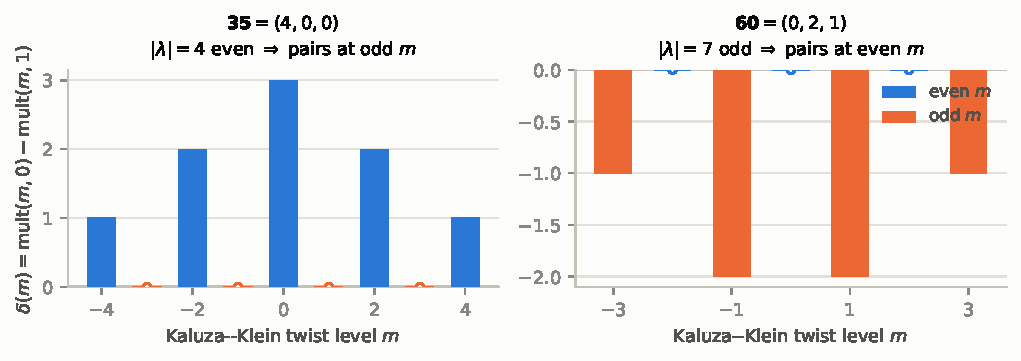
\includegraphics[width=\textwidth]{fig_combs.pdf}
\caption{La dicotomía, vista directamente. El desequilibrio con signo
$\delta(m)=\mathrm{mult}(m,0)-\mathrm{mult}(m,1)$ para el fermión de AHMN (izquierda) y para
la representación más pequeña capaz de alojar una generación de quarks (derecha). Cada uno es
un \emph{peine}: uno se anula en todo diente par, el otro en todo diente impar, y qué peine le
toca a una representación lo decide un único bit, la paridad de su carga del centro. Los
marcadores huecos se sitúan sobre los dientes que se anulan idénticamente. Ninguna
representación tiene ambos peines llenos, y fuera de la clase $\mathcal Z$ de
\S\ref{sec:degenerate} ninguna los tiene ambos vacíos.}
\label{fig:combs}
\end{figure}

La Figura~\ref{fig:combs} es el corolario con el álgebra quitada. Dos observaciones fijan el
significado. Primera, $\lam=a+2b+3c\equiv a+c \pmod 2$, de modo que la paridad en cuestión es
exactamente la puerta~1 de la Parte~II --- y es el \emph{cociente} $\ZZ_2$ de la carga del
centro $\ZZ_4$, no la carga del centro misma. Segunda, la misma paridad ya venía haciendo
trabajo silencioso en la Parte~II: el recuento de modos cero quirales $N=(b+1)(a+c+1)/2$ es
entero solo porque $a+c$ es impar siempre que la carga del centro es impar, una observación
entre paréntesis allí. Tres apariciones, en tres sectores que no comparten coordenada: la
puerta de admisibilidad, la integralidad del recuento de modos cero, y ahora el equilibrio de
twists de la torre. Es el invariante el que hace el trabajo, no el marco.

\paragraph{La muesca es un hueco, no una cancelación.} Vale la pena ver qué le hace el
Corolario~\ref{cor:dichotomy} al potencial mismo, porque el enunciado es más concreto que
``las multiplicidades se equilibran''. Expandiendo $V$ en modos de Fourier sobre el toro, la
amplitud en el vector de frecuencia $m\,(k_1,k_2)$ --- el $m$-ésimo armónico en la
dirección $(k_1,k_2)$ --- porta el factor
$\sum_q\mathrm{mult}(m,q)\,(-1)^{k_2q}$, que es la multiplicidad \emph{total} cuando $k_2$ es
par y exactamente $\delta(m)$ cuando $k_2$ es impar. La muesca no orquesta por tanto una
cancelación delicada entre contribuciones: vacía una subred entera del espacio de Fourier.
Para una representación de carga del centro impar, \emph{todo} modo con $k_2$ impar y $m$ par
está idénticamente ausente del potencial --- no pequeño, ausente. La
Figura~\ref{fig:spectrum} muestra a las ocho representaciones admisibles dejando vacíos
exactamente los mismos asientos, y al $\mathbf{35}$ de AHMN llenando los $95$.

\begin{figure}[p]
\centering
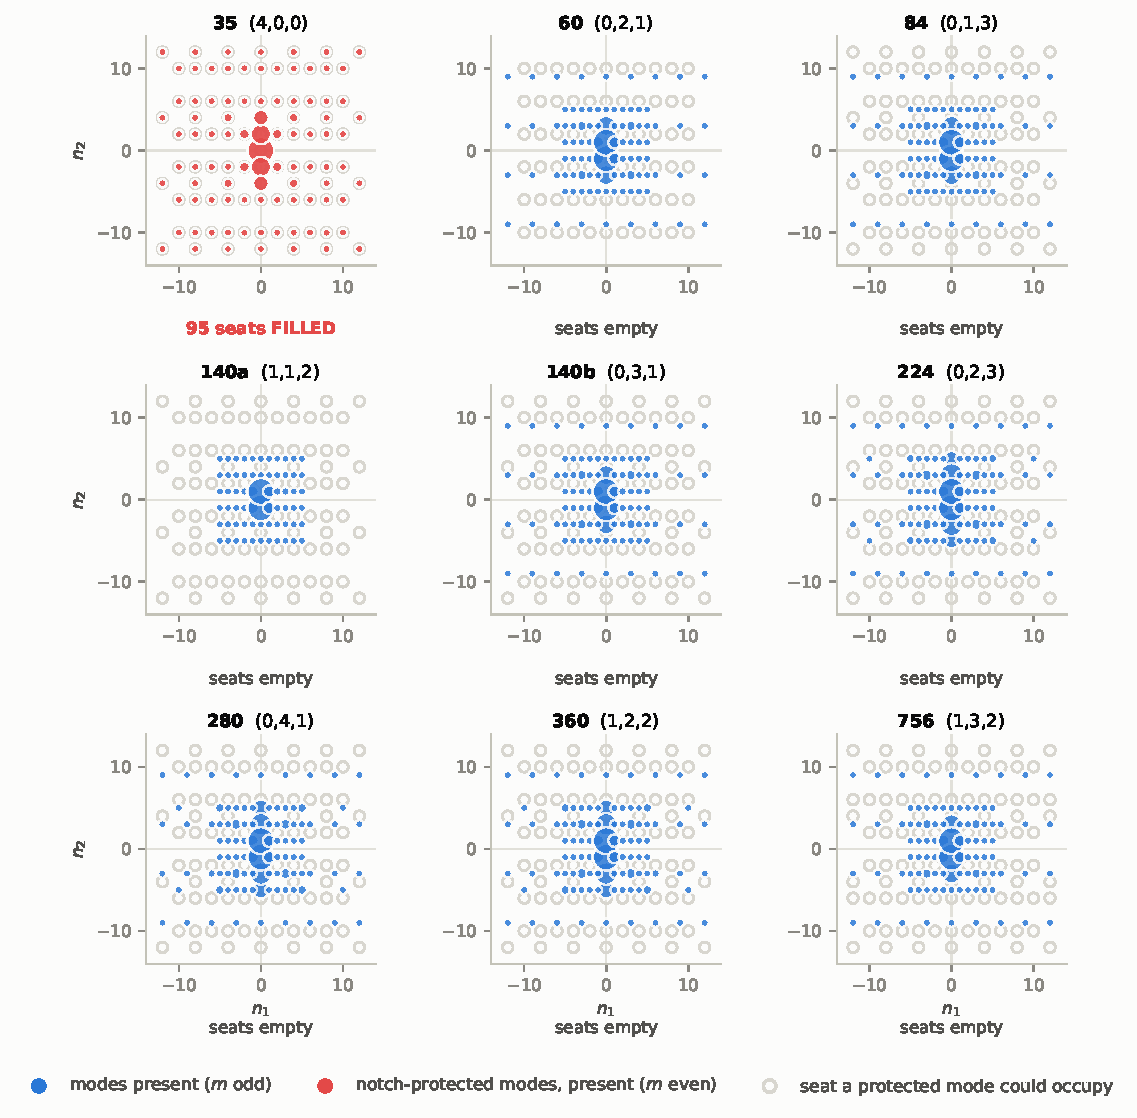
\includegraphics[width=0.93\textwidth]{fig_spectrum.pdf}
\caption{\textbf{La muesca, vista como ausencia.} Cada panel es el plano de Fourier del
potencial a un loop para una representación, restringido a las capas de $k_2$ impar --- el
sector cuya amplitud es $\delta(m)$. Los discos rellenos son modos que el potencial porta de
hecho, con tamaño según la amplitud; los anillos huecos marcan cada asiento que un modo
\emph{protegido por la muesca} ($m$ par) podría ocupar. Ocho representaciones dejan todos esos
asientos vacíos, y son exactamente las ocho que pueden alojar una generación de quarks del
Modelo Estándar. La novena, el $\mathbf{35}$ de AHMN, los llena. Nada se ajustó ni se
umbralizó: los asientos vacíos son ceros exactos, y el patrón es el único bit
$a{+}2b{+}3c \bmod 2$ hecho visible.}
\label{fig:spectrum}
\end{figure}

\emph{Establecido aquí:} exactamente uno de los dos emparejamientos se cumple, cuál lo decide
la paridad de la carga del centro, y la consecuencia es una subred idénticamente vacía del
soporte de Fourier del potencial. \emph{Abierto:} la clase degenerada donde se cumplen ambos
y --- el motivo del trabajo --- qué hace ya el caso de $m$ impar en la literatura.

% ===================================================================
\section{La clase degenerada}\label{sec:degenerate}
El Corolario~\ref{cor:dichotomy} calla cuando $D$ se anula idénticamente. Esa clase es
pequeña, exactamente calculable --- y su existencia es la huella de un grupo que no es conexo.

$O(n)$ tiene dos componentes, y todo lo incómodo de su teoría de representaciones desciende
de ahí. Sus representaciones irreducibles vienen en pares \emph{asociados} $\mu$ y
$\mu\otimes\det$, indistinguibles sobre las rotaciones y opuestos sobre las reflexiones;
algunos son su propio compañero. Como los diagramas de Young se construyeron para $GL$ y
$S_n$, etiquetar con ellos las representaciones de $O(n)$ produce etiquetas ``no estándar'' que
hay que reparar, y Newell escribió las reglas de reparación en 1951~\cite{Newell}, con King
sistematizándolas para las tres familias clásicas dos décadas después~\cite{King71}. La
incomodidad no es puntillismo contable; es la desconexión asomando a través de la notación.
La influyente reformulación de Koike y Terada la resuelve del modo más limpio posible ---
trabajando en $R(SO(n))$ y tratando las etiquetas de $O(n)$ como una base~\cite{KoikeTerada} ---
lo cual es elegante, universalmente usado y, para nuestros fines, precisamente el movimiento
equivocado: identificar $\mu$ con $\mu\otimes\det$ es exactamente la información que
necesitamos.

Ese es el sentido en que existe la clase de abajo. Consiste en las representaciones cuya
ramificación es \emph{ciega} a la reflexión --- autoasociadas de cabo a rabo, de modo que
toda contribución se cancela contra una compañera. La física la vio primero, como una torre
con ambos peines vacíos.

\begin{teorema}[Clase degenerada]\label{thm:Z}
$D\equiv0$ si y solo si
\[
\boxed{\;b\ \text{impar}\ \wedge\ \big[(a,c\ \text{ambos impares})\ \vee\ (a=c\ \text{par})\big]\;}
\]
En consecuencia la muesca de $m$ par se cumple si y solo si $a+2b+3c$ es impar o
$(a,b,c)\in\mathcal Z$, y como todo miembro de $\mathcal Z$ tiene $\lam$ par, $\mathcal Z$ es
disjunta de la clase que satisface la puerta de la Parte~II.
\end{teorema}

\begin{proof}[Esbozo de demostración]
Escribe $D=N/V$ con $N=\det(y_i^{\mu_j})$ el bialternante sobre el alfabeto ordenado
$y=(1,-1,t,t^{-1})$ y $\mu=(a{+}b{+}c{+}3,\;b{+}c{+}2,\;c{+}1,\;0)$. Expande $N$ por Laplace
a lo largo de las dos filas \emph{constantes}: el menor $2\times2$ sobre las columnas $j<k$
es $(-1)^{\mu_k}-(-1)^{\mu_j}$, de modo que solo sobreviven columnas de $\mu$-paridad
opuesta, mientras que todo menor complementario sobre las filas $(t,t^{-1})$ vale
$[\mu_l-\mu_m]$ con $[x]:=t^x-t^{-x}$. Las ocho clases de paridad de $(a,b,c)$ caen en cuatro
tipos. Si todos los $\mu_j$ son pares --- es decir, $a,b,c$ todos impares --- todo menor
superviviente se anula y $N\equiv0$. Si exactamente un $\mu_j$ tiene la paridad minoritaria,
$N$ es una combinación de tres corchetes cuyo mayor argumento es la suma de los otros dos, y
por tanto no puede cancelarse. De las tres clases con una división de paridad dos-dos, dos
contienen el corchete $[P]$ con $P=a{+}b{+}c{+}3$ estrictamente mayor que todo otro
argumento, así que tampoco hay cancelación; la tercera, $a,c$ pares y $b$ impar, da
$N/2=[Q]-[R]+[P{-}Q]-[P{-}R]$ con los cuatro argumentos positivos, que se anula si y solo si
$\{Q,P{-}Q\}=\{R,P{-}R\}$ como multiconjuntos, y como $Q=R$ forzaría $b=-1$ esto ocurre si y
solo si $a=c$. El único input analítico es que $\{[x]\}_{x>0}$ es linealmente independiente,
que es el enunciado de que monomios distintos son independientes.
\end{proof}

El teorema está verificado de cuatro modos independientes --- multiplicidades de peso de
Weyl, un barrido exacto de bialternantes sobre $10\,648$ representaciones hasta
$(a,b,c)\le21$ sin discrepancia alguna, comprobaciones simbólicas de cada fórmula de caso, y
una auditoría adversarial --- y certificado en Lean~4 (Cuadro~\ref{tab:lean}). La
Figura~\ref{fig:landscape} pone el teorema y el criterio de la Parte~II sobre la misma lámina:
$\mathcal Z$ ocupa sus propias celdas y nunca se encuentra con una representación capaz de
alojar una generación de quarks, que es la disjunción del Corolario~\ref{cor:dichotomy} vista
en vez de deducida.

\begin{figure}[t]
\centering
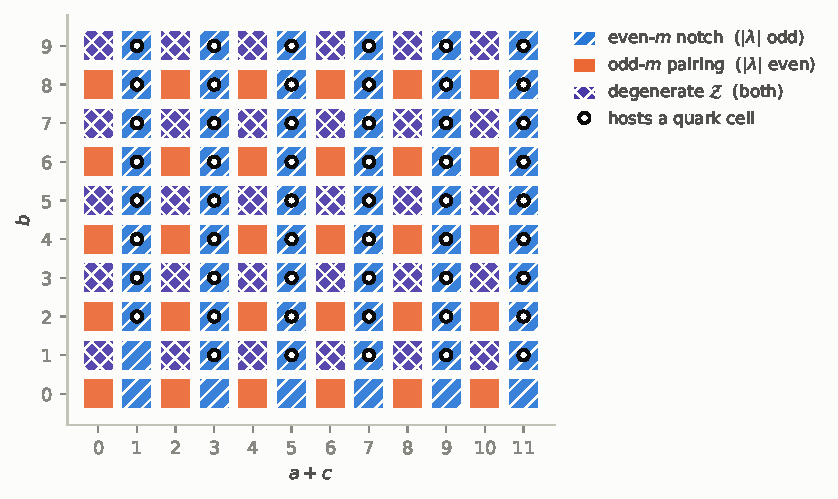
\includegraphics[width=0.92\textwidth]{fig_landscape_notch.pdf}
\caption{El paisaje entero en una lámina. Cada celda es un par de etiquetas $(a+c,\,b)$ --- las
dos coordenadas de las que la clasificación depende realmente --- coloreada según qué
emparejamiento satisface la torre. La paridad de columna azul es la puerta~1 de la Parte~II
disfrazada: esas son precisamente las representaciones que pueden alojar una generación de
quarks, anilladas allí donde las dos cláusulas restantes ($b\ge1$, $a+b+c\ge3$) también se
cumplen. Las celdas violeta son la clase degenerada $\mathcal Z$ del Teorema~\ref{thm:Z}, que
satisface ambos emparejamientos y, como la figura hace visible, nunca toca un anillo. Todo lo
de este trabajo es un enunciado sobre la frontera entre el azul y el naranja.}
\label{fig:landscape}
\end{figure}

\begin{table}[t]
\centering\small
\begin{tabular}{p{5.7cm}p{8.4cm}}
\toprule
\rowcolor{hdrblue}
\textcolor{white}{Teorema en Lean (\texttt{NotchCentreCharge.lean})} & \textcolor{white}{contenido}\\
\midrule
\texttt{notch\_degenerate\_iff} &
$N\,a\,b\,c=0 \leftrightarrow (\mathrm{Odd}\,b \wedge ((\mathrm{Odd}\,a\wedge \mathrm{Odd}\,c)\vee a=c))$ --- Teorema~\ref{thm:Z}, sobre
$\ZZ[T;T^{-1}]$, sin \texttt{decide} sobre el determinante\\
\midrule
\rowcolor{softgrey}
\texttt{notch\_parity} &
Lema~\ref{lem:parity} como identidad libre de divisiones sobre el bialternante\\
\midrule
\texttt{degenerate\_centre\_charge\_even} &
todo miembro de $\mathcal Z$ tiene $a+2b+3c$ par\\
\midrule
\rowcolor{softgrey}
\texttt{degenerate\_disjoint\_admissible} &
$\lam$ impar $\Rightarrow N\neq0$; las dos clases nunca se encuentran\\
\bottomrule
\end{tabular}
\caption{El núcleo verificado por máquina. Todos los enunciados están libres de
\texttt{sorry} y dependen solo de \texttt{propext}, \texttt{Classical.choice},
\texttt{Quot.sound}. El paso de independencia lineal se sustituye por la extracción de un
único coeficiente de Laurent en el argumento de corchete estrictamente mayor, que es finita y
efectiva.}
\label{tab:lean}
\end{table}

\paragraph{Qué es nuevo aquí y qué no.} El mecanismo es clásico y lo decimos con claridad. El
alfabeto $\{1,-1,t,t^{-1}\}$ tiene determinante $-1$, de modo que es el elemento semisimple
genérico de la componente \emph{impropia} $O(4)^-$; una representación irreducible de $O(4)$
y su asociada $\mu\otimes\det$ tienen allí caracteres opuestos, y toda
$\mu=(\mu_1,\mu_2)$ con $\mu_2\ge1$ es autoasociada y no contribuye
nada~\cite[Thm.~5]{Brauer}. Por tanto $D\equiv0$ si y solo si el multiconjunto de
ramificación de Littlewood de $\lambda$ es estable bajo la involución de asociación, es
decir, si y solo si $c^\lambda_{(m)}=c^\lambda_{(m,1,1)}$ para todo $m\ge1$ y
$c^\lambda_\varnothing=c^\lambda_{(1^4)}$. Nuestra demostración \emph{es} ese cálculo en otra
base: se comprueba $V=-2[1]^3$, de modo que los corchetes $[x]$ son los caracteres de la
componente impropia $\chi^-_{(x-1)}$ salvo normalización. Damos la ruta del bialternante
porque evita la contabilidad de modificaciones --- la regla de Littlewood no está modificada
solo para $\ell(\lambda)\le n/2=2$, esto es, solo para $c=0$, y fuera de ese rango se
requieren las reglas de modificación de King~\cite{King71,Newell,Brauer}, apareciendo etiquetas
ilegales de $O(4)$ con multiplicidad ya para etiquetas tan pequeñas como $(2,1,2)$. Eso es una
ventaja práctica, no conceptual. Lo que reclamamos es la clasificación aritmética explícita
en etiquetas de Dynkin y su certificado en Lean, no el fenómeno ni la técnica.

\emph{Establecido aquí:} $\mathcal Z$ exactamente, disjunta de la clase admisible de la
Parte~II. \emph{Abierto:} si la clasificación es corolario de algún criterio general de
componente impropia; no hemos hallado ninguno, y \S\ref{sec:ledger} registra dónde miramos.

% ===================================================================
\section{El precio: un dominio fundamental que no se transfiere}\label{sec:domain}
Aquí está el giro. La mitad de $m$ impar del Corolario~\ref{cor:dichotomy} no es una
curiosidad nuestra. Es una hipótesis ya en uso --- y sostiene el argumento.

Al calcular el potencial a un loop de la línea de Wilson, AHMN reducen la región de búsqueda.
Observan~\cite[\S4.3]{AHMN}, en el original:
\begin{quote}\itshape
``For odd $m$, the spectrum with $(m,q)=(m,1)$ at a given $\alpha_2$ is equivalent to that
with $(m,q)=(m,0)$ at $\alpha_2+1$. Hence, if the effective potential contains an equal
number of KK mode with $(m,0)$ and $(m,1)$ for odd $m$, their combined contribution is also
periodic under $\alpha_2\to\alpha_2+1$.''
\end{quote}
La dan luego por satisfecha mediante inspección --- \emph{``From Table~1, we see that\dots''} ---
para su propio contenido de campos, y obtienen la región
fundamental~\cite[Ec.~(4.15)]{AHMN}
\begin{equation}\label{eq:region}
0\le\alpha_1<1,\qquad 0\le\alpha_2\le\tfrac12 .
\end{equation}
Su comprobación es correcta. Pero la hipótesis no es una propiedad de su modelo; por el
Corolario~\ref{cor:dichotomy} es una propiedad de la \emph{representación}, y se invierte con
la carga del centro. La Tabla~\ref{tab:flip} es el argumento entero.

\begin{table}[t]
\centering\small
\begin{tabular}{lccc c}
\toprule
\rowcolor{hdrblue}
\textcolor{white}{sector} & \textcolor{white}{$(a,b,c)$} & \textcolor{white}{$\lam$} &
\textcolor{white}{hipótesis de AHMN ($m$ impar)} & \textcolor{white}{muesca de $m$ par}\\
\midrule
adjunto gauge $\mathbf{15}$ & $(1,0,1)$ & $4$ par & sí & no\\
\rowcolor{softgrey}
fermión de AHMN $\mathbf{35}$ & $(4,0,0)$ & $4$ par & sí & no\\
\textbf{toda rep.\ admisible} & puerta~1 & \textbf{impar} & \textbf{no} & \textbf{sí}\\
\bottomrule
\end{tabular}
\caption{La inversión. La puerta~1 de la Parte~II fuerza $\lam$ impar para cualquier
representación capaz de alojar una generación de quarks, mientras que el adjunto gauge es
inevitablemente par --- de modo que los dos sectores caen en paridades opuestas y ninguna
completación admisible puede restaurar el emparejamiento en $m$ impar que
necesita~\eqref{eq:region}.}
\label{tab:flip}
\end{table}

Para el espectro total dependiente del valor esperado de vacío, gauge más fermión, la
precondición de~\eqref{eq:region} se cumple para el $\mathbf{35}$ y falla para cada una de
las ocho representaciones admisibles de dimensión $\le400$.

La Tabla~\ref{tab:vsahmn} pone los dos argumentos uno junto al otro, porque la relación entre
ellos es fácil de malinterpretar. No contradecimos un resultado; identificamos la hipótesis que
hay debajo, mostramos que esa hipótesis es una propiedad de la representación y no del modelo,
y observamos que se invierte sobre la clase que uno querría usar a continuación.

\begin{table}[t]
\centering\small
\begin{tabular}{p{2.5cm}p{4.6cm}p{4.3cm}p{3.0cm}}
\toprule
\rowcolor{hdrblue}
\textcolor{white}{} & \textcolor{white}{hipótesis} & \textcolor{white}{estado de esa hipótesis} & \textcolor{white}{conclusión extraída}\\
\midrule
AHMN~\cite{AHMN} \S4.3 &
multiplicidades iguales de $(m,0)$ y $(m,1)$ en $m$ \textbf{impar} &
comprobada inspeccionando su Tabla~1, para su propio contenido de campos &
$\alpha_2\in[0,\tfrac12]$ \eqref{eq:region}\\
\midrule
\rowcolor{softgrey}
este trabajo, \S\ref{sec:dichotomy} &
ninguna --- el emparejamiento se \emph{deriva} &
un teorema: qué peine le toca a una representación es $(a{+}2b{+}3c)\bmod2$ &
la dicotomía, Cor.~\ref{cor:dichotomy}\\
\midrule
consecuencia &
la Parte~II fuerza $\lam$ impar en toda rep.\ admisible; el adjunto gauge es par &
el emparejamiento en $m$ impar falla en toda la clase física, verificado sobre $V$ mismo &
$\alpha_2\in[0,1]$: el toro completo, Cor.~\ref{cor:domain}\\
\bottomrule
\end{tabular}
\caption{La relación con el resultado sobre el que este trabajo se apoya. El argumento de AHMN
es correcto y su comprobación válida para su modelo; lo que no estaba disponible entonces es
que su hipótesis la decide la carga del centro, y que por tanto se invierte exactamente sobre
las representaciones capaces de alojar el Modelo Estándar.}
\label{tab:vsahmn}
\end{table}

\paragraph{La conclusión, contrastada en vez de inferida.} AHMN demuestran
\emph{emparejamiento $\Rightarrow$ periodo~$1$}. Mostrar que el emparejamiento falla no
muestra por sí solo que falle la periodicidad --- eso sería negar el antecedente, y podría
existir otra ruta hacia la misma periodicidad. Así que contrastamos la conclusión
directamente sobre el potencial. Evaluando $V$ sobre el toro de periodo~$2$ por transformada
rápida de Fourier (es exactamente una serie de cosenos bidimensional, ya que $k_2q$ es entero
y el término de seno muere) y comparando $V(\alpha_1,\alpha_2{+}1)$ con
$V(\alpha_1,\alpha_2)$:

\begin{center}\footnotesize
\begin{tabular}{lccccccccc}
\toprule
\rowcolor{hdrblue}
\textcolor{white}{rep} & \textcolor{white}{$\mathbf{35}$} & \textcolor{white}{$\mathbf{60}$} &
\textcolor{white}{$\mathbf{84}$} & \textcolor{white}{$\mathbf{140}a$} & \textcolor{white}{$\mathbf{140}b$} &
\textcolor{white}{$\mathbf{216}$} & \textcolor{white}{$\mathbf{224}$} & \textcolor{white}{$\mathbf{280}$} &
\textcolor{white}{$\mathbf{360}$}\\
\midrule
$\max|V(\alpha_2{+}1)-V|/\text{escala}$ & $\mathbf{0}$ & $0.30$ & $0.21$ & $0.045$ & $0.12$ &
$0.12$ & $0.095$ & $0.19$ & $0.023$\\
\bottomrule
\end{tabular}
\end{center}

\begin{figure}[t]
\centering
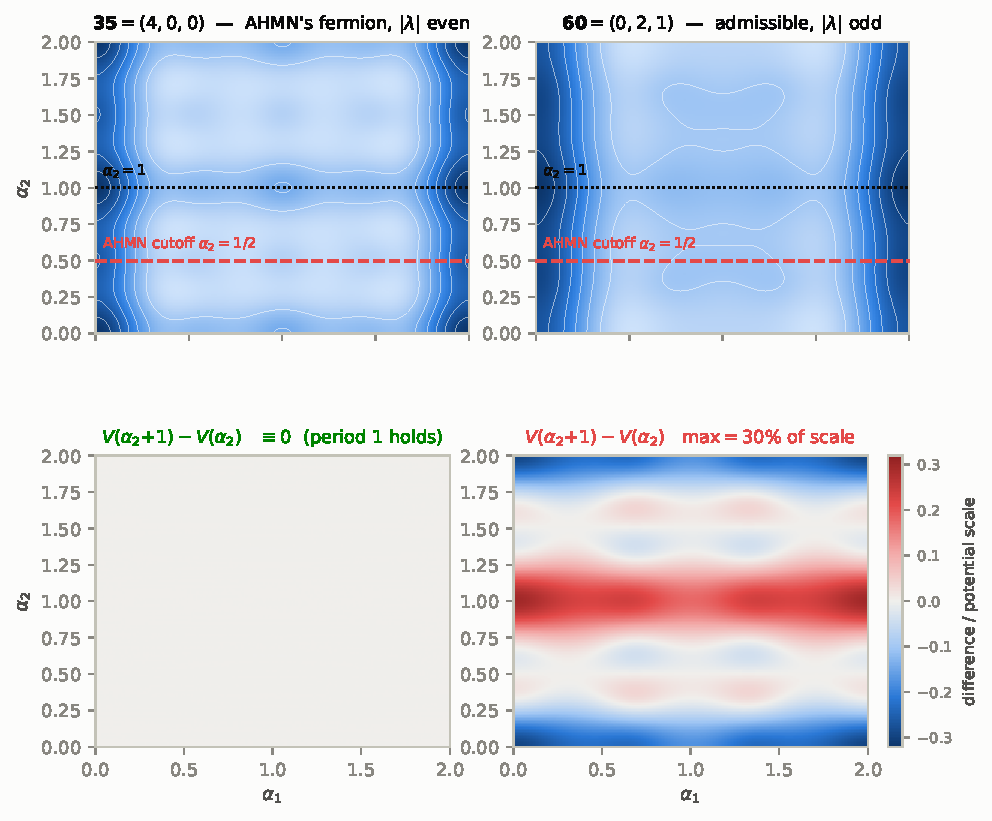
\includegraphics[width=\textwidth]{fig_domain.pdf}
\caption{La afirmación central, sin álgebra. \textbf{Arriba:} el potencial a un loop de la
línea de Wilson sobre el toro completo de periodo~$2$, para el fermión de AHMN (izquierda) y
para la representación admisible más pequeña (derecha); la línea discontinua es el borde de la
región fundamental~\eqref{eq:region} que usa la literatura. \textbf{Abajo:} el test directo,
$V(\alpha_1,\alpha_2{+}1)-V(\alpha_1,\alpha_2)$ en la misma escala. A la izquierda es
\emph{idénticamente cero} --- gris plano, la periodicidad se cumple y el medio dominio es
legal. A la derecha es un $30\%$ estructurado de la propia amplitud del potencial. Nada del
panel derecho es más pequeño, más sutil o más numérico que el izquierdo; la simetría
sencillamente no está, y toda representación candidata capaz de alojar el Modelo Estándar
está en ese lado.}
\label{fig:domain}
\end{figure}

El $\mathbf{35}$ es de periodo~$1$ \emph{exactamente}; toda representación admisible lo viola
en un $2$--$30\%$ de la propia escala del potencial --- una cantidad física, no ruido
numérico (Figura~\ref{fig:domain}). La reflexión $\alpha_2\to-\alpha_2$ sí sobrevive en las
nueve. De ahí que para las representaciones admisibles la región fundamental sea
$\alpha_2\in[0,1]$: exactamente el doble que la de AHMN.

\begin{corolario}\label{cor:domain}
La reducción~\eqref{eq:region} no se transfiere del modelo de AHMN a ninguna representación
admisible para el Modelo Estándar. Una minimización para tal representación debe barrer el
toro completo; una búsqueda restringida al medio dominio puede devolver un punto de frontera
que no es un vacío.
\end{corolario}

\paragraph{Y ninguna otra identificación lo rescata.} Agrandar un dominio fundamental invita
a la objeción obvia: quizá alguna \emph{otra} identificación, no considerada aquí, vuelva a
encogerlo. Sobre un toro los candidatos naturales son las transformaciones modulares, que
actúan sobre las fases de la línea de Wilson mezclando los dos ciclos --- el mismo grupo que
organiza el programa de simetría de sabor modular~\cite{Feruglio,RatzEclectic}. Medimos por
tanto, en vez de suponer, qué transformaciones del retículo respeta $V$ realmente. El grupo
superviviente es exactamente $\{\alpha_1\to\pm\alpha_1\}\times\{\alpha_2\to\pm\alpha_2\}$
junto con las traslaciones: las reflexiones y $S^2=-\mathbf{1}$ se cumplen hasta el cero de
máquina para toda representación contrastada, mientras que la propia $S$, el intercambio
$\alpha_1\leftrightarrow\alpha_2$ y la cizalla $\alpha_1\to\alpha_1+\alpha_2$ están todas
rotas a orden unidad. Es lo que cabe esperar de~\eqref{eq:U}: $U_5=\mathbf{1}$ mientras
$U_6\neq\mathbf{1}$, de modo que los dos ciclos son inequivalentes y nada que los mezcle puede
sobrevivir a la proyección del orbifold. La consecuencia para nosotros es que
$\alpha_2\in[0,1]$ no es meramente mayor que~\eqref{eq:region} --- es la región fundamental
correcta y \emph{completa}, sin ninguna identificación adicional disponible para reducirla.

Vale la pena señalar un residuo, más que interpretarlo. La cizalla
$\alpha_2\to\alpha_1+\alpha_2$ está rota, pero por un margen que cae monótonamente con la
dimensión de la representación: $0.24$, $0.18$, $0.13$, $0.075$ y $0.027$ para el
$\mathbf{35}$, $\mathbf{60}$, $\mathbf{84}$, $\mathbf{216}$ y $\mathbf{360}$
respectivamente. Si eso es una recuperación asintótica de una simetría modular en el límite
de representación grande, o meramente el suavizado del potencial al contribuir más modos, no
lo sabemos; una única sucesión monótona no es evidencia, y lo enunciamos solo como
observación.

Esto no es una fe de erratas para~\cite{AHMN}, cuyo contenido de campos satisface su propia
hipótesis. Es un aviso para todo lo que viene después: el paso siguiente natural en este
programa --- meter una representación realista que aloje quarks en la maquinaria de AHMN ---
pierde silenciosamente una simetría que las convenciones de esa maquinaria suponen. Lo pagamos
nosotros mismos. Una versión anterior de nuestra propia ordenación por naturalidad se calculó
sobre el medio dominio, y su minimizador quedaba clavado a la frontera $\alpha_2=\tfrac12$ en
cinco de nueve representaciones; lo diagnosticamos como un defecto de implementación y lo
arreglamos numéricamente. No era un defecto. Era una simetría heredada que nuestras
representaciones no tienen.

\emph{Establecido aquí:} la reducción a medio dominio se invierte sobre la clase física,
verificado sobre el potencial mismo. \emph{Abierto:} qué recibe la clase admisible \emph{a
cambio} --- el asunto de la sección siguiente, y no lo que uno adivinaría.

% ===================================================================
\section{Qué compra la muesca: un desacoplamiento exacto}\label{sec:decoupling}
El emparejamiento en $m$ impar compra periodicidad. La muesca de $m$ par compra algo bastante
distinto, y la diferencia es la razón de que una ordenación por naturalidad en esta clase haya
sido tan difícil de estabilizar.

La forma de lo que sigue resulta familiar de otro contexto. Appelquist y Carazzone demostraron
que los estados pesados desaparecen de los observables de baja energía salvo correcciones
suprimidas~\cite{AppelquistCarazzone}, y la lección absorbida desde entonces tiene doble filo:
lo que está protegido frente a un observable es también \emph{invisible} para él. Una cantidad
a la que una simetría prohíbe contribuir no puede medirse por aquello a lo que no contribuye.
Lo que hallamos abajo es una versión discreta y exacta de ese intercambio. La muesca no
suprime la contribución de la representación fermiónica a un observable concreto; la aniquila.
Y el precio es exactamente el que los lectores de Appelquist y Carazzone aprendieron a
esperar: ese observable ya no puede distinguir una representación de otra.

El orden dominante de Kaluza--Klein de la curvatura en $\alpha_2$ en el punto medio está
construido \emph{enteramente} a partir del desequilibrio de $m$ par
$\delta(m):=\mathrm{mult}(m,0)-\mathrm{mult}(m,1)$:
\begin{equation}\label{eq:Dstruct}
\mathcal D\;=\;\pi^2\Big(\sum_{m\equiv2\,(4)}m^2\delta(m)\;-\;\sum_{m\equiv0\,(4)}m^2\delta(m)\Big).
\end{equation}
Pero la muesca es precisamente el enunciado $\delta(m)=0$ para todo $m$ par. Por tanto:

\begin{corolario}[Desacoplamiento]\label{cor:decoupling}
Para toda representación admisible para el Modelo Estándar, la contribución del sector
fermiónico a $\mathcal D$ se anula idénticamente. $\mathcal D$ se reduce al sector gauge solo
--- el mismo número para toda representación admisible, independiente de $(a,b,c)$.
\end{corolario}

Numéricamente, $\mathcal D=-27.6$ para las ocho representaciones admisibles, idéntico hasta el
dígito, mientras que el no admisible $\mathbf{35}$, que rompe la muesca, queda aparte en
$-185.5$. Esta es la forma familiar de una ley de conservación: lo que hace de la muesca un
\emph{detector} limpio de admisibilidad la hace ciega como \emph{discriminador} entre
representaciones admisibles.

\paragraph{Una inferencia refutada, registrada a propósito.} Es tentador concluir de
$\mathcal D<0$ uniformemente que $\alpha_2=\tfrac12$ es una cresta de curvatura para toda
representación admisible. Esa inferencia es falsa, y la registramos porque el fallo es
instructivo. Contra la curvatura verdadera (convergida, $K_{\max}=16$):

\begin{center}\footnotesize
\begin{tabular}{lccccccccc}
\toprule
\rowcolor{hdrblue}
\textcolor{white}{rep} & \textcolor{white}{$\mathbf{35}$} & \textcolor{white}{$\mathbf{60}$} &
\textcolor{white}{$\mathbf{84}$} & \textcolor{white}{$\mathbf{140}a$} & \textcolor{white}{$\mathbf{140}b$} &
\textcolor{white}{$\mathbf{216}$} & \textcolor{white}{$\mathbf{224}$} & \textcolor{white}{$\mathbf{280}$} &
\textcolor{white}{$\mathbf{360}$}\\
\midrule
$\mathcal D$ (orden dominante) & $-185.5$ & $-27.6$ & $-27.6$ & $-27.6$ & $-27.6$ & $-27.6$ & $-27.6$ & $-27.6$ & $-27.6$\\
\rowcolor{softgrey}
$\partial^2_{\alpha_2}V$ real en $\tfrac12$ & $-200.6$ & $+21.2$ & $-5.8$ & $-85.1$ & $-188.6$ & $+255.2$ & $-160.4$ & $+16.8$ & $+245.5$\\
el signo coincide & sí & \textbf{no} & sí & sí & sí & \textbf{no} & sí & \textbf{no} & \textbf{no}\\
\bottomrule
\end{tabular}
\end{center}

El proxy de orden dominante predice mal el signo en cuatro de ocho. Acierta en el
$\mathbf{35}$ --- la única representación donde el sector fermiónico lo domina, y el caso
contra el que tal proxy queda implícitamente calibrado. Se validó en el único régimen donde
funciona y se aplicó luego en el régimen donde la muesca le ha quitado el contenido.

\paragraph{La consecuencia que importa.} Juntando ambas cosas:

\begin{quote}
La muesca no fija el signo de la curvatura en $\alpha_2$; \emph{aniquila el término
dominante}. Para toda representación admisible el orden dominante de Kaluza--Klein es
degenerado --- idéntico, puramente gauge. Todo lo que distingue una representación admisible
de otra vive en los términos subdominantes.
\end{quote}

Esto explica desde la teoría, y no desde la autopsia, por qué una ordenación por naturalidad
sobre esta clase es delicada: los candidatos son indistinguibles a orden dominante \emph{por
un teorema}, y la cantidad que los separa es exactamente la que peor resuelve una minimización
gruesa. Junto con el Corolario~\ref{cor:domain}, los dos modos de fallo conocidos de tal
cálculo son consecuencias del mismo cambio de paridad.

\emph{Establecido aquí:} un desacoplamiento exacto, y el origen estructural de la fragilidad.
\emph{Abierto:} la propia estructura subdominante --- que ahora tiene diana, ya que el orden
dominante se conoce en forma cerrada y es una constante.

% ===================================================================
\section{Medir el espacio en vez del punto}\label{sec:basin}
Toda fragilidad de arriba viene de evaluar en un punto: un minimizador clavado a una frontera,
una curvatura leída en esa frontera, un hessiano tomado por diferencias finitas, un autovalor
casi nulo en una dirección plana. El único enunciado exacto de este trabajo --- la muesca ---
es un enunciado sobre el contenido de Fourier completo de $V$ sobre el toro. Esa asimetría
sugiere cambiar de instrumento.

Para un pozo cuadrático el conjunto de subnivel $S(\varepsilon)=\{V<V_{\min}+\varepsilon\Delta V\}$
es una elipse de semiejes $\sqrt{2\varepsilon\Delta V/\lambda_i}$, y una elipse uniforme tiene
tensor de segundo momento $M_{ii}=a_i^2/4$. Ambos autovalores de curvatura se siguen por tanto
de una \emph{integral} sobre la cuenca,
\begin{equation}
\lambda_i=\frac{\varepsilon\,\Delta V}{2\,M_{ii}},
\end{equation}
sin derivadas y sin paso. Se requieren dos correcciones y ambas se hallaron contrastando en
vez de razonando: $\varepsilon$ debe estar en el régimen cuadrático (en $\varepsilon=0.15$ el
conjunto de subnivel cubre un $40$--$76\%$ del toro y $M$ satura contra el toro mismo, leyendo
una anisotropía genuina de $413{:}1$ como $1.17{:}1$), y $S(\varepsilon)$ debe restringirse a
la componente conexa del mínimo global, ya que el toro porta mínimos equivalentes por simetría
y un conjunto sin restringir mide la separación \emph{entre} mínimos --- siendo la firma
$\lambda\propto\varepsilon$ en vez de una meseta.

Corregida, la medida tiene una meseta en $\varepsilon\in[3\cdot10^{-4},10^{-3}]$ que reproduce
el hessiano por diferencias finitas para ocho de nueve representaciones. En la novena ---
$(0,3,1)$, aquella donde las diferencias finitas no son de fiar --- la deriva bajo
$K_{\max}\!:\,4\to14$ cae del $68.9\%$ al $0.6\%$. Dos hechos establecidos por el camino
merecen registrarse: la \emph{ubicación} del vacío está ya convergida en $K_{\max}=4$
(idéntica a cuatro decimales hasta $K_{\max}=14$; el $\mathbf{35}$ cae en $(0.4360,0.2986)$
contra el $(0.438,0.299)$ citado por AHMN, lo que confirma la calibración), de modo que la
falta de convergencia nunca afectó a dónde está el vacío, solo a la curvatura allí; y el modo
bajo de $(0,3,1)$ es genuinamente \emph{anarmónico}, sin meseta en $\varepsilon$ en absoluto,
de modo que una masa cuadrática es sencillamente el descriptor equivocado para esa dirección
en vez de uno difícil de medir.

\emph{Establecido aquí:} un reemplazo integral del hessiano, validado allí donde el hessiano es
fiable y estable allí donde no lo es. \emph{Abierto:} la propia ordenación subdominante.

% ===================================================================
\section{Una comprobación previa, y quién debería ejecutarla}\label{sec:tool}
La Parte~I terminó empaquetando su teorema de Existencia como un oráculo reutilizable en vez
de dejarlo como una afirmación sobre un modelo. Vale la pena hacer lo mismo aquí, porque el
Corolario~\ref{cor:domain} no es un hecho sobre $(3,\mathbf{60})$ --- es una comprobación que
cualquiera que construya sobre esta clase de construcción debería ejecutar \emph{antes} de
gastar tiempo de máquina.

\paragraph{Para qué sirve.} La reducción~\eqref{eq:region} es el tipo de paso que viaja como
convención. Aparece una vez, se justifica una vez para un contenido de campos, y a partir de
ahí se hereda --- razonablemente, ya que rederivar cada dominio fundamental haría ilegible la
literatura. El problema es que su hipótesis depende de la representación y se invierte
exactamente sobre las representaciones que uno querría usar a continuación. Una minimización
corrida sobre la región reducida a la mitad para tal representación no falla ruidosamente;
devuelve un punto de frontera que parece un vacío. Ese modo de fallo es silencioso, y por eso
merece una herramienta y no una observación.

\paragraph{Qué hace.} \texttt{notch\_preflight.py} toma o bien etiquetas de Dynkin o bien una
tabla explícita de multiplicidades $(m,q)$, e informa de qué emparejamiento satisface la
torre, qué región fundamental es por tanto legal, y si la representación puede alojar una
celda de quarks siquiera. Sobre etiquetas aplica directamente el Corolario~\ref{cor:dichotomy} y
el Teorema~\ref{thm:Z}; sobre una tabla \emph{mide} ambos emparejamientos en vez de suponer
ninguno, de modo que sigue siendo válida para espectros fuera del marco de $SU(4)$ donde
nuestro teorema se aplica. Salida típica:

\begin{center}\small
\begin{tabular}{ll}
\toprule
\rowcolor{hdrblue}
\textcolor{white}{\texttt{notch\_preflight.py 0 2 1}} & \textcolor{white}{\texttt{notch\_preflight.py 4 0 0}}\\
\midrule
centre charge: odd & centre charge: even\\
\rowcolor{softgrey}
tower pairs at: even $m$ & tower pairs at: odd $m$\\
odd-$m$ hypothesis: \textcolor{warmred}{\textbf{FAILS}} & odd-$m$ hypothesis: \textcolor{okgreen}{\textbf{HOLDS}}\\
\rowcolor{softgrey}
legal region: $\alpha_2\in[0,1]$ \textbf{(full torus)} & legal region: $\alpha_2\in[0,\tfrac12]$\\
hosts a quark cell: \textbf{yes} & hosts a quark cell: no\\
\bottomrule
\end{tabular}
\end{center}

\paragraph{Quién debería ejecutarla.} Cualquiera que extienda un modelo gauge--Higgs de
orbifold a una nueva representación de materia, antes de minimizar; cualquiera que reutilice
un dominio fundamental publicado con un contenido de campos distinto; y cualquiera que
encuentre un minimizador posándose repetidamente sobre una frontera del dominio --- que, como
registra \S\ref{sec:domain}, es el aspecto que tiene una simetría ausente vista desde dentro.
La comprobación no cuesta nada: es un bit de paridad.

\emph{Establecido aquí:} la consecuencia operativa del trabajo como comprobación ejecutable.
\emph{Abierto:} la misma pregunta para otros grupos de orbifold, donde el alfabeto
de~\eqref{eq:D} cambia y la dicotomía debe rederivarse en vez de reutilizarse --- exactamente
el error que esta herramienta existe para prevenir.

% ===================================================================
\section{Balance}\label{sec:ledger}
Como en la Parte~II exponemos la autoría punto por punto en vez de en prosa; el
Cuadro~\ref{tab:ledger} es esa contabilidad.

\begin{table}[h]
\centering\small
\begin{tabular}{p{4.0cm}p{5.0cm}p{5.2cm}}
\toprule
\rowcolor{hdrblue}
\textcolor{white}{Elemento} & \textcolor{white}{Heredado (citar)} & \textcolor{white}{Nuestro}\\
\midrule
congruencia de carga del centro &
$n$-alidad $\ZZ_4$; $Y$ fraccionaria atada al centro~\cite{Hucks,Saller,Tong,Alonso,Slansky} &
nada --- como en la Parte~II, no reclamamos nada de ello\\
\midrule
\rowcolor{softgrey}
orbifold, twists $(m,q)$, potencial a un loop, Ec.~\eqref{eq:region} &
AHMN~\cite{AHMN} &
la derivación de $(m,q)$ desde las condiciones de contorno, y la lectura por multipletes de la Tabla~1\\
\midrule
lema de paridad~\ref{lem:parity} &
elemental (simetría + homogeneidad de $s_\lambda$) & presentado como observación, no como resultado\\
\midrule
\rowcolor{softgrey}
mecanismo de $D\equiv0$ &
asociada/twist por $\det$ de $O(2n)$; restricción de Littlewood; reglas de modificación de King~\cite{King71,Newell,Brauer,AyyerBehrend} &
la clasificación aritmética explícita (Tma.~\ref{thm:Z}) y su certificado en Lean\\
\midrule
la dicotomía, Cor.~\ref{cor:dichotomy} & --- & nuestra\\
\midrule
\rowcolor{softgrey}
inversión de \eqref{eq:region}, Cor.~\ref{cor:domain} & --- & nuestra, y verificada directamente sobre el potencial\\
\midrule
desacoplamiento, Cor.~\ref{cor:decoupling} & --- & nuestro\\
\bottomrule
\end{tabular}
\caption{Qué debe cada resultado. La novedad de \S\ref{sec:degenerate} es un enunciado, no un
fenómeno ni una técnica; la novedad de \S\S\ref{sec:domain}--\ref{sec:decoupling} es la
física.}
\label{tab:ledger}
\end{table}

\paragraph{Dónde miramos.} Buscando un criterio general que decida cuándo un carácter de
$GL(n)$ se anula idénticamente sobre $O(n)^-$ --- del cual el Teorema~\ref{thm:Z} sería
corolario --- leímos Koike--Terada~\cite{KoikeTerada}, King~\cite{King71b},
Littlewood~\cite{Littlewood58}, Fauser--Jarvis--King--Wybourne~\cite{FJKW},
Ayyer--Kumari~\cite{AyyerKumari}, Kumari~\cite{Kumari}, Ayyer--Behrend~\cite{AyyerBehrend} y
Albion~\cite{Albion}, y no hallamos ninguno. Koike--Terada no puede contenerlo: definen
$R(O(n))$ como subanillo de $R(SO(n))$, y como $V_\mu$ y $V_\mu\otimes\det$ restringen a la
misma irreducible de $SO(n)$, la involución de asociación queda cocientada antes de que la
pregunta pueda plantearse. Un vecino cercano merece separación explícita: el Ejemplo~2.16 de
Ayyer--Kumari enuncia un criterio de paridad de $O(4)$ en $(x,-x)$, que parece idéntico al
nuestro y no lo es --- su elemento del toro tiene determinante $+1$, la componente
\emph{propia}. Dos fuentes clásicas quedan sin leer y las señalamos como tales: el trabajo de
King de 1971 sobre reglas de modificación en su propia exposición, y el libro de Littlewood,
Cap.~XI.

% ===================================================================
\section{Reflexiones}\label{sec:reflections}
\paragraph{Una convención heredada porta una hipótesis no enunciada.} La
Ecuación~\eqref{eq:region} viaja como convención --- un dominio fundamental, de esas cosas que
uno copia sin rederivar. Su hipótesis justificante no viaja con ella, y en este caso la
hipótesis se invierte exactamente sobre la clase que uno querría usar a continuación.
Sospechamos que no es un caso aislado en la construcción de modelos de orbifold, donde
dominios fundamentales, asignaciones $Z_2$ y reducciones ``sin pérdida de generalidad'' se
heredan rutinariamente entre trabajos con contenidos de campos distintos. La protección barata
es llevar la hipótesis como comprobación ejecutable en vez de como observación.

\paragraph{El centro como restricción sobre el potencial, no sobre la materia.} El cambio de
punto de vista es fácil de perder entre los corolarios, así que lo enunciamos sin rodeos.

Durante cincuenta años el centro del grupo gauge se ha usado en una sola dirección. La
cuantización de Dirac, las fases de 't~Hooft, la lectura que Hucks y Saller hacen del propio
$\ZZ_6$ del Modelo Estándar: en todas ellas el centro es una condición sobre \emph{qué
representaciones pueden existir}, o portar qué cargas. La Parte~II también lo usó así, y lo
dijo. El centro restringe la materia.

Lo que hemos hallado es que en una construcción gauge--Higgs el mismo invariante restringe
además el \emph{potencial}. No haciendo pequeña alguna contribución: eliminando idénticamente
un sector de Fourier entero del potencial de Hosotani, para toda representación de la paridad
equivocada. El Higgs en estos modelos es una línea de Wilson; un periodo de línea de Wilson es
una transformación gauge central; de modo que el centro actúa sobre el sector de Higgs con la
misma inmediatez con que actúa sobre el sector de materia, y su carga decide qué puede
aparecer allí. La Figura~\ref{fig:spectrum} es ese enunciado dibujado: para ocho de nueve
representaciones, una subred de armónicos especificada aritméticamente no es pequeña, está
vacía.

Lo diríamos así. La carga del centro se ha leído como una puerta sobre la materia. Es también
una puerta sobre el potencial, y las dos puertas abren en direcciones opuestas --- que es por
lo que la condición que permite a una representación alojar el Modelo Estándar es la misma
condición que le niega a su potencial de línea de Wilson una simetría que la literatura viene
suponiendo.

\paragraph{Una conjetura, enunciada para poder matarla.} El mecanismo que sabemos demostrar es
específico de $SU(4)$ en su aritmética pero no en su lógica, y es más útil decir qué esperamos
que detenerse en lo que calculamos.

\begin{quote}
\emph{Conjetura (selección por paridad del centro, forma general).} Sea un modelo gauge--Higgs
de orbifold cuyo espectro de Kaluza--Klein tiene etiquetas de twist capturadas por un carácter
$\chi_\lambda$ evaluado sobre un alfabeto $A$, al modo de~\eqref{eq:D}. Supóngase que un
desplazamiento unidad de un módulo de línea de Wilson lleva $A$ a $\zeta\cdot A$ salvo un
elemento de Weyl, para algún $\zeta$ del centro del grupo gauge, de orden $d$. Entonces los
armónicos del potencial a un loop se escinden en $d$ sectores etiquetados por la carga del
centro módulo $d$, y los sectores en que $\zeta^{\,c(R)}\neq1$ están idénticamente ausentes
del potencial de una representación $R$.
\end{quote}

Demostramos el caso $d=2$, en el modelo donde todo ingrediente puede calcularse exactamente, y
verificamos la precondición estructural a lo largo de $SU(N)$ más abajo. Lo que no hemos hecho
es exhibir un segundo modelo, de $d$ distinta, en el que los sectores aparezcan como se
predice; ese es el test obvio y el modo obvio de matar esto. Un orbifold $\ZZ_N$ con $N>2$, o
una línea de Wilson cuyo desplazamiento unidad realice un elemento central de orden tres, lo
zanjaría en un solo cálculo.

\paragraph{¿Es esto un accidente de $SU(4)$?} Es la primera pregunta que cabe hacerle
a~\eqref{eq:principle}, y tiene una respuesta afilada y no meramente esperanzada.

El principio necesita que el desplazamiento iguale a un elemento central \emph{salvo Weyl}, que
es la condición de multiconjuntos $-A=A|_{t\to-t}$ sobre el alfabeto
$A=\{\varepsilon_i\,t^{c_i}\}$, con $\varepsilon_i=\pm1$ procedente del twist $\ZZ_2$ y $c_i$
la carga bajo la línea de Wilson. Separemos las posiciones según $c_i$. Las de $c_i=\pm1$
satisfacen la condición automáticamente, ya que $-\varepsilon t^{\pm1}$ y
$\varepsilon(-1)^{\pm1}t^{\pm1}$ son el mismo monomio. Las de $c_i=0$ no: la negación les
cambia el signo y nada en $t$ puede deshacerlo, de modo que han de emparejarse, un $+1$ contra
un $-1$. \emph{Las posiciones neutras frente a la línea de Wilson deben portar signos de twist
equilibrados}, y en particular ha de haber un número par de ellas.

Para una única dirección de línea de Wilson eso significa $N-2$ par, y por tanto $N$ par. Un
barrido por fuerza bruta sobre todos los alfabetos de esta forma lo confirma:

\begin{center}\small
\begin{tabular}{lcccccc}
\toprule
\rowcolor{hdrblue}
\textcolor{white}{$SU(N)$} & \textcolor{white}{$N{=}3$} & \textcolor{white}{$N{=}4$} &
\textcolor{white}{$N{=}5$} & \textcolor{white}{$N{=}6$} & \textcolor{white}{$N{=}7$} &
\textcolor{white}{$N{=}8$}\\
\midrule
alfabetos que admiten la regla & $0$ & $192$ & $0$ & $4880$ & $0$ & $134400$\\
\rowcolor{softgrey}
posiciones neutras cuando se cumple & --- & $2$ & --- & $4$ & --- & $6$\\
veredicto & ninguno & \textbf{existe} & ninguno & \textbf{existe} & ninguno & \textbf{existe}\\
\bottomrule
\end{tabular}
\end{center}

Así pues, el mecanismo no es ni un accidente ni universal: vive sobre los grupos unitarios
pares, y \textbf{$SU(4)$ es el grupo más pequeño capaz de portarlo}. Los grupos impares quedan
excluidos por una razón que se enuncia en una frase --- un número impar de posiciones
espectadoras no puede equilibrar sus signos de twist --- y esa razón es estructural, no
numérica.

Dos límites honestos del barrido. Supone la forma de AHMN: un único twist $\ZZ_2$ que aporta
signos, y una única dirección de línea de Wilson con cargas en $\{0,\pm1\}$. Un orbifold
$\ZZ_N$, o una línea de Wilson con cargas mayores, cambia la condición --- el elemento central
relevante ya no tiene por qué ser de orden dos, y la congruencia que aparecería sería módulo
su orden y no módulo $2$. No hemos barrido esos casos, y no los reclamamos.

\paragraph{El método es una sombra.} Vale la pena nombrar lo que de hecho se hizo, porque el
mismo movimiento está disponible en otros sitios. Nada en este trabajo estudia una
representación de $SU(4)$ directamente. Lo que estudia es una \emph{sombra}: la
especialización $D(t)=s_\lambda(1,-1,t,t^{-1})$ colapsa un sistema de pesos cuadridimensional
sobre un único polinomio de Laurent, y el orbifold es quien elige el muro sobre el que
proyectar --- las dos paridades $\ZZ_2$ y la línea de Wilson fijan el alfabeto, y no nos toca
a nosotros escogerlo. Leídos así, los resultados son enunciados sobre sombras. La dicotomía
(Corolario~\ref{cor:dichotomy}) dice que la sombra es siempre simétrica, con la carga del
centro decidiendo respecto a qué eje. La muesca dice que la sombra tiene huecos, en posiciones
aritméticamente exactas --- y la Figura~\ref{fig:spectrum} son esos huecos. La clase degenerada
$\mathcal Z$ del Teorema~\ref{thm:Z} es la más extraña de las tres: esas representaciones no
proyectan \emph{sombra alguna} sobre este muro. No son pequeñas --- $\mathcal Z$ contiene
representaciones de todo tamaño --- y desde aquí son sencillamente invisibles, que es por lo
que la física nunca las ve y por lo que hubo que clasificarlas por álgebra en vez de hallarlas
por inspección.

La moraleja práctica es que el muro te lo eligen. Una proyección de orbifold distinta es un
alfabeto distinto en~\eqref{eq:D}, y por tanto una sombra distinta y una dicotomía distinta;
eso es precisamente por lo que \S\ref{sec:tool} advierte contra reutilizar el resultado en vez
de rederivarlo. Lo que generaliza no es la respuesta sino la pregunta: dada una
compactificación, pregunta qué especialización impone sobre el carácter, y lee la física en la
sombra.

\paragraph{Una puerta puede ser un filtro.} La imagen que emerge es que la representación
actúa como un \emph{filtro} sobre la onda del vacío: $V(\alpha)$ es una serie de Fourier en la
línea de Wilson, la suma de Kaluza--Klein es una transformada de Fourier sobre el toro oculto,
y el espectro de multiplicidades de la representación decide qué componentes pasan. El
Corolario~\ref{cor:decoupling} dice que las representaciones admisibles son precisamente
aquellas cuyo filtro es ciego a orden dominante --- elegir una representación capaz de alojar
el Modelo Estándar instala automáticamente una muesca en su propio potencial de Higgs. Si esa
ceguera es una molestia o un principio de diseño (elegir la representación para conformar el
filtro) es la pregunta que más nos gustaría responder a continuación.

\paragraph{El orden dominante es una constante, así que apunta por debajo.} Como el
Corolario~\ref{cor:decoupling} fija el término dominante en forma cerrada, el problema de
naturalidad está ahora bien planteado en vez de meramente ser difícil: calcular la estructura
subdominante con un gradiente analítico y control explícito de convergencia, contra un orden
dominante que se sabe degenerado. Esa es una tarea más afilada que hacer más cuidadoso un
minimizador, y es la primera vez que hay razón para esperar que sea necesaria.

% ===================================================================
\section{Conclusión}\label{sec:conclusion}
La Parte~II identificó su primera puerta como clásica y la regaló. Este trabajo muestra que la
puerta hacía más trabajo que el sector en que se halló, y la razón cabe en una frase: avanzar
la línea de Wilson un período es, salvo una reflexión de Weyl, multiplicar por el elemento
central $-\mathbf{1}$, de modo que el centro actúa sobre el sector de Higgs con la misma
inmediatez con que actúa sobre el sector de materia. Una representación responde con un solo
bit, y ese bit decide qué armónicos del potencial de Hosotani tienen permitido existir. Lo que
durante cincuenta años se ha leído como una restricción sobre \emph{qué representaciones
pueden portar qué cargas} es también una restricción sobre \emph{qué puede contener el
potencial}.

En concreto: la paridad de la carga del centro
$\ZZ_4$ --- equivalentemente $a+c$ --- decide cuál de dos emparejamientos de twist de
Kaluza--Klein satisface una representación, y ambos son mutuamente excluyentes fuera de una
clase degenerada explícitamente clasificada. Uno de esos emparejamientos es la hipótesis bajo
la cual la literatura de gauge--Higgs con dos dobletes reduce a la mitad su dominio fundamental
de línea de Wilson; el otro es lo que toda representación admisible para el Modelo Estándar
tiene en su lugar. La consecuencia es concreta y, creemos, inevitable para el programa: la
reducción a medio dominio no se transfiere, hay que barrer el toro completo, y el orden
dominante de Kaluza--Klein de la curvatura en el punto medio es independiente de la
representación, de modo que cualquier ordenación de candidatos por naturalidad es un enunciado
sobre términos subdominantes, se presente o no como tal.

No reclamamos nada de la congruencia de carga del centro, exactamente como antes. Lo que
reclamamos es que no es solo una puerta sobre la materia: es una puerta sobre el potencial, y
las dos puertas abren en direcciones opuestas. De un testigo, a la ley de elegibilidad, al
descubrimiento de que la cláusula más clásica de la ley gobierna el sector por el que nunca se
le preguntó --- ese es el arco de los tres trabajos.

\paragraph{Disponibilidad de datos y reproducibilidad.} Todos los scripts, datos de pesos,
fuentes de Lean~4 y código de generación de figuras se proporcionan como ficheros anexos;
ningún dato más allá de lo que ellos generan sustenta afirmación alguna aquí. Todo número se
regenera desde los scripts anexos: el barrido de bialternantes del Teorema~\ref{thm:Z}, la
fuente en Lean~4 de la Tabla~\ref{tab:lean}, la derivación de $(m,q)$ y la comprobación de
reparto de multipletes de \S\ref{sec:projection}, el test directo de periodicidad de
\S\ref{sec:domain}, el desacoplamiento y la comparación de curvaturas de
\S\ref{sec:decoupling}, y la medida de cuenca de \S\ref{sec:basin} con sus barridos en
$\varepsilon$ y $K_{\max}$.

\begin{thebibliography}{99}
\bibitem{PartI} C.~Mar\'in, \emph{Anomaly- and Tadpole-Compatible Fermion Completion of
Six-Dimensional $SU(4)$ Gauge--Higgs Unification} (Parte~I), Zenodo (2026),
DOI:\,10.5281/zenodo.21429144.
\bibitem{PartII} C.~Mar\'in, \emph{Three Gates to a Quark Generation} (Parte~II), Zenodo
(2026), DOI:\,10.5281/zenodo.21432628.
\bibitem{SSSW} C.A.~Scrucca, M.~Serone, L.~Silvestrini, A.~Wulzer, \emph{Gauge-Higgs
Unification in Orbifold Models}, JHEP \textbf{02} (2004) 049, hep-th/0312267.
\bibitem{AHMN} K.~Akamatsu, T.~Hirose, N.~Maru, A.~Nago, \emph{Two Higgs Doublet Model from
Gauge--Higgs Unification in Six Dimensions}, arXiv:2603.05857.
\bibitem{Slansky} R.~Slansky, \emph{Group theory for unified model building},
Phys.\ Rept.\ \textbf{79} (1981) 1.
\bibitem{Hucks} J.~Hucks, \emph{Global structure of the standard model, anomalies, and
charge quantization}, Phys.\ Rev.\ D \textbf{43} (1991) 2709.
\bibitem{Saller} M.~Saller, \emph{The Central Correlations of Hypercharge, Isospin, Colour
and Chirality in the Standard Model}, Nuovo Cim.\ A \textbf{111} (1998) 1375,
arXiv:hep-th/9802112.
\bibitem{Tong} D.~Tong, \emph{Line Operators in the Standard Model}, JHEP \textbf{07}
(2017) 104, arXiv:1705.01853.
\bibitem{Alonso} R.~Alonso, D.~Dimakou, J.~West, \emph{Fractional-charge hadrons and
leptons to tell the Standard Model group apart}, arXiv:2404.03438.
\bibitem{Brauer} A.~Solymos, D.~Jakab, Z.~Zimbor\'as, \emph{Extendibility of Brauer states},
arXiv:2411.04597. (Prop.~1 and Thms.~5, 9 of App.~A give, in modern notation, the Littlewood
restriction rule, the $O(2k)$ self-associate fact, and the Newell--King modification rules.)
\bibitem{King71} R.C.~King, \emph{Modification Rules and Products of Irreducible
Representations of the Unitary, Orthogonal, and Symplectic Groups}, J.\ Math.\ Phys.\
\textbf{12} (1971) 1588.
\bibitem{King71b} R.C.~King, \emph{Branching rules for classical Lie groups using tensor and
spinor methods}, Can.\ J.\ Math.\ \textbf{23} (1971) 176.
\bibitem{Newell} M.J.~Newell, \emph{Modification rules for the orthogonal and symplectic
groups}, Proc.\ Roy.\ Irish Acad.\ \textbf{54} (1951) 153.
\bibitem{Littlewood58} D.E.~Littlewood, \emph{Products and plethysms of characters with
orthogonal, symplectic and symmetric groups}, Can.\ J.\ Math.\ \textbf{10} (1958) 17.
\bibitem{KoikeTerada} K.~Koike, I.~Terada, \emph{Young-diagrammatic methods for the
representation theory of the classical groups of type $B_n$, $C_n$, $D_n$},
J.\ Algebra \textbf{107} (1987) 466.
\bibitem{FJKW} B.~Fauser, P.D.~Jarvis, R.C.~King, B.G.~Wybourne, \emph{New branching rules
induced by plethysm}, J.\ Phys.\ A \textbf{39} (2006) 2611, arXiv:math-ph/0505037.
\bibitem{AyyerKumari} A.~Ayyer, N.~Kumari, \emph{Factorization of classical characters
twisted by roots of unity}, J.\ Algebra \textbf{609} (2022) 437, arXiv:2109.11310.
\bibitem{Kumari} N.~Kumari, \emph{Factorization of classical characters twisted by roots of
unity: II}, arXiv:2212.12477.
\bibitem{AyyerBehrend} A.~Ayyer, R.E.~Behrend, \emph{Factorization theorems for classical
group characters, with applications to alternating sign matrices and plane partitions},
J.\ Combin.\ Theory Ser.\ A \textbf{165} (2019) 78, arXiv:1804.04514.
\bibitem{Albion} S.P.~Albion, \emph{Universal characters twisted by roots of unity},
arXiv:2212.07343.
\bibitem{tHooft} G.~'t~Hooft, \emph{On the phase transition towards permanent quark
confinement}, Nucl.\ Phys.\ B \textbf{138} (1978) 1.
\bibitem{ScherkSchwarz} J.~Scherk, J.H.~Schwarz, \emph{Spontaneous breaking of supersymmetry
through dimensional reduction}, Phys.\ Lett.\ B \textbf{82} (1979) 60.
\bibitem{Manton} N.S.~Manton, \emph{A new six-dimensional approach to the Weinberg--Salam
model}, Nucl.\ Phys.\ B \textbf{158} (1979) 141.
\bibitem{Fairlie} D.B.~Fairlie, \emph{Higgs' fields and the determination of the Weinberg
angle}, Phys.\ Lett.\ B \textbf{82} (1979) 97.
\bibitem{Hosotani} Y.~Hosotani, \emph{Dynamical mass generation by compact extra
dimensions}, Phys.\ Lett.\ B \textbf{126} (1983) 309.
\bibitem{KawamuraGUT} Y.~Kawamura, \emph{Triplet-doublet splitting, proton stability and
extra dimension}, Prog.\ Theor.\ Phys.\ \textbf{105} (2001) 999, arXiv:hep-ph/0012125.
\bibitem{AppelquistCarazzone} T.~Appelquist, J.~Carazzone, \emph{Infrared singularities and
massive fields}, Phys.\ Rev.\ D \textbf{11} (1975) 2856.
\bibitem{Weyl} H.~Weyl, \emph{The Classical Groups: Their Invariants and Representations},
Princeton University Press (1939).
\bibitem{LittlewoodBook} D.E.~Littlewood, \emph{The Theory of Group Characters and Matrix
Representations of Groups}, 2nd ed., Oxford University Press (1950).
\bibitem{Murnaghan} F.D.~Murnaghan, \emph{The Theory of Group Representations}, Johns
Hopkins Press (1938).
\bibitem{HoweTanWillenbring} R.~Howe, E.-C.~Tan, J.F.~Willenbring, \emph{Stable branching
rules for classical symmetric pairs}, Trans.\ Amer.\ Math.\ Soc.\ \textbf{357} (2005) 1601,
arXiv:math/0311159.
\bibitem{CiucuKrattenthaler} M.~Ciucu, C.~Krattenthaler, \emph{A factorization theorem for
classical group characters, with applications to plane partitions and rhombus tilings},
arXiv:0812.1251.
\bibitem{Feruglio} F.~Feruglio, \emph{Are neutrino masses modular forms?}, in
\emph{From My Vast Repertoire: Guido Altarelli's Legacy}, World Scientific (2019) 227,
arXiv:1706.08749.
\bibitem{RatzEclectic} H.P.~Nilles, S.~Ramos-S\'anchez, P.K.S.~Vaudrevange, \emph{Eclectic
flavor groups}, JHEP \textbf{02} (2020) 045, arXiv:2001.01736; véase también M.~Ratz et al.\
para el desarrollo de la simetría de sabor modular basado en orbifolds.
\end{thebibliography}
\end{document}
